%% =============================================================================
%% IST submission — Overleaf package (flat layout)
%%
%% Build on Overleaf (pdfLaTeX + BibTeX, default settings):
%%   pdflatex main
%%   bibtex main
%%   pdflatex main && pdflatex main
%%
%% Files (paths relative to main.tex):
%%   main.tex
%%   cap3_article_body.tex
%%   cover_letter.tex
%%   results/qa_assessment_summary.tex
%%   results/kappa/kappa_report.tex
%%   results/auxiliary/aux_qa_summary.tex
%%   results/auxiliary/aux_ft_summary.tex
%%   results/auxiliary/aux_reft_summary.tex
%%   results/auxiliary/kappa/aux_kappa_report.tex
%%   results/ec5_recovery/ec5_recovery_report.tex
%%   results/sensitivity/sensitivity_report.tex
%%   results/final_review/missing_references.bib
%%   results/segress_checklist.tex
%%   results/human_validation/human_kappa_report.tex
%%   results/human_validation/human_confusion_report.tex
%% =============================================================================

\documentclass[review,3p,times]{elsarticle}

%% --- Math + tables ---
\usepackage{amsmath,amssymb}
\usepackage{booktabs}
\usepackage{multirow}
\usepackage{array}
\usepackage{tabularx}
\usepackage{makecell}
\usepackage{longtable}
\usepackage{caption}

%% --- Figures ---
\usepackage{graphicx}
\usepackage{tikz}
\usetikzlibrary{arrows.meta,positioning,shapes,calc}
\usepackage{pgfplots}
\pgfplotsset{compat=1.18}

%% --- Misc ---
\usepackage{enumitem}
\usepackage{xcolor}
\usepackage{hyperref}
\hypersetup{colorlinks=true, linkcolor=blue!50!black, citecolor=blue!50!black, urlcolor=blue!50!black,
  pdftitle={Process Mining and Stochastic Modeling for Software Process Forecasting: A Systematic Mapping Study with a Human-Checked LLM-Assisted Screen},
  pdfauthor={Rodrigo Almeida de Oliveira, Juliano de Paulo Ribeiro, Edson Emilio Scalabrin}}
%% Suppress the author-markup tokens elsarticle feeds to the PDF author string.
\makeatletter
\pdfstringdefDisableCommands{\let\corref\@gobble \let\fnref\@gobble \let\comma\@empty \let\@fnmark\@empty \let\@corref\@empty \let\cnotenum\@empty}
\makeatother
%% IST asks for line numbers in the review version.
\usepackage{lineno}
\modulolinenumbers[5]
%% Allow DOI/URL strings to wrap inside table cells (pdflatex).
\usepackage{xurl}

%% --- Bibliography style: Elsevier numeric + sorted ---
\bibliographystyle{elsarticle-num}

%% --- Zenodo replication-package DOI (new deposit, 2026-08-14) ---
\newcommand{\zenododoi}{10.5281/zenodo.21939600}
\newcommand{\zenododoiurl}{https://doi.org/\zenododoi}

%% --- Round-2 placeholders: filled after `python -m pipeline.round2_validation --compute`.
%% Must not remain in the submitted PDF: `grep -n "\tbd" *.tex` must return nothing.
\newcommand{\tbd}[1]{\textcolor{red}{\textbf{[#1]}}}

\journal{Information and Software Technology}

\begin{document}
\linenumbers

%% =========================
%% Front matter
%% =========================
\begin{frontmatter}

\title{Process Mining and Stochastic Modeling for Software Process
       Forecasting: A Systematic Mapping Study with a Human-Checked
       LLM-Assisted Screen}

%% Authors
\author[pucpr]{Rodrigo Almeida de Oliveira\corref{cor1}\fnref{orcid1}}
\ead{rodrigo.almeida1@pucpr.edu.br}

\author[pucpr]{Juliano de Paulo Ribeiro\fnref{orcid2}}
\ead{juliano.ribeiro@pucpr.edu.br}

\author[pucpr]{Edson Emilio Scalabrin\fnref{orcid3}}
\ead{scalabrin@ppgia.pucpr.br}

\cortext[cor1]{Corresponding author.}

\fntext[orcid1]{ORCID: 0009-0009-6310-4126}
\fntext[orcid2]{ORCID: 0009-0004-3605-485X}
\fntext[orcid3]{ORCID: 0000-0002-3918-1799}

\affiliation[pucpr]{
  organization={Pontif\'icia Universidade Cat\'olica do Paran\'a (PUCPR), Graduate Program in Informatics (PPGIa)},
  city={Curitiba},
  state={PR},
  country={Brazil}
}

%% --- Abstract (150–300 words, structured) ---
\begin{abstract}
\textbf{Context.}
Process mining (PM) and stochastic models can turn software process
event data into forecasts of software development lifecycle (SDLC)
metrics. No secondary study maps their joint use on software development
data.
\textbf{Objective.}
To assemble and classify a corpus at that intersection, to measure the
selection error of an LLM-assisted screen against a pre-registered human
reference, and to propose a research agenda.
\textbf{Method.}
A systematic mapping study reported against
SEGRESS~\cite{kitchenham2023segress}. Searches of five databases on
12~April~2026 yielded 5{,}783 deduplicated records. An LLM screened
them in two tiers; two human raters checked the screen on pre-registered
samples against a bar of Recall $\geq 0.90$ and re-screened the records
the LLM had excluded. Studies
read from an abstract or a PDF were classified into four technique and
data families.
\textbf{Results.}
Recall is 0.630 on the working-set sample (29 of 46; Wilson 95\% CI
0.486--0.755) and 0.725 (235 of 324) on the auxiliary tier, both below
the bar. Three failure mechanisms are named: a second pass that read the
abstract rather than the PDF, records without an abstract closed by rule,
and 32 includes (9.5\% of 338) whose title or abstract does not support
inclusion. The human re-screen added 150 studies; the corpus is 456. On
the 151 working-set studies with full family codes, 104 match process
mining, 49 a stochastic model, and 27 forecasting; one study in the 380
with family marks matches all three.
\textbf{Conclusion.}
The family codes describe named cuts of this corpus, not the rate at
which the literature combines the three techniques. The SPMF taxonomy and
the agenda are proposals by the authors; the PATHCAST pipeline is future
work.
\textbf{Limitations.}
The second pass used the abstract for almost every record; 76 added
studies were read from the title alone; free-text extraction fields are
withdrawn (0\% exact match with a human rater on 31 studies).
\end{abstract}

\begin{keyword}
Systematic Mapping Study \sep
Process Mining \sep
Stochastic Modeling \sep
Software Process Forecasting \sep
LLM-Assisted Screening \sep
Mining Software Repositories
\end{keyword}

%% --- Highlights (3–5 bullets, ≤85 chars each) ---
\begin{highlights}
\item Pre-registered human check of an LLM screen: Recall 0.630 and 0.725 vs a 0.90 bar.
\item Three failure mechanisms of the screen are named and quantified.
\item Corpus of 456 studies at the PM, stochastic, and forecasting intersection.
\item One study (PRIMAD) joins process mining, stochastic modelling, and forecasting.
\item Replication package: Zenodo DOI 10.5281/zenodo.21939600.
\end{highlights}

\end{frontmatter}

%% =========================
%% Body
%% =========================
\section{Introduction}
\label{sec:slr-intro}

Software organisations routinely need to answer forecasting questions about
their own development process: when a feature will be delivered, how long an
issue will remain open, or whether a release will slip. The data needed to
answer them already exists as a by-product of everyday work---commits, issue
transitions, pull requests, code reviews, and CI/CD executions are all
time-stamped events. Three research communities have developed techniques
that can exploit these traces, largely independently of one another.
\emph{Process mining} (PM) discovers, checks, and enhances process models
from event logs, and has been applied to software repositories since the
work of Cook and Wolf~\cite{cook1995,cook1998} and Rubin et
al.~\cite{rubin2007}. \emph{Stochastic modelling}---Markov chains,
stochastic Petri nets, Monte Carlo simulation---has a long tradition in
software reliability and process simulation~\cite{whittaker1994,ali2014simulation}.
\emph{Machine-learning-based prediction} dominates mining-software-repositories
research on defects, effort, and outcomes~\cite{kagdi2007msr,hall2012fault},
and, in the business-process domain, predictive process
monitoring~\cite{marquezchamorro2018predictive}. Combining them is attractive
because each covers a weakness of the others: PM provides an empirically
grounded process structure, stochastic models turn that structure into
probability distributions over future paths and durations, and ML can
correct systematic errors using context features. Whether, and how far, the
literature has actually combined them for software processes is not known.

\paragraph{Related secondary studies.} Existing secondary studies each cover
one side of this space. In business process management, predictive process
monitoring has been surveyed and benchmarked for outcome
prediction~\cite{teinemaa2019outcome}, remaining-time
prediction~\cite{verenich2019remaining}, and in
general~\cite{marquezchamorro2018predictive}, but on business event logs
rather than software development processes. General mappings of process
mining applications~\cite{garcia2019pmmapping,thiede2018pmorg} treat software
engineering as one domain among many and do not address forecasting. Within
software engineering, secondary studies have covered process simulation
modelling~\cite{zhang2010simulation,ali2014simulation}, process mining of
FLOSS event logs~\cite{mukala2015floss}, software process mining with Petri
nets~\cite{thamizharasan2016petri}, continuous software monitoring backed by
process mining~\cite{stepanov2026continuous}, repository
mining~\cite{kagdi2007msr}, and defect prediction~\cite{hall2012fault}. Four
of these (\cite{zhang2010simulation,mukala2015floss,thamizharasan2016petri,stepanov2026continuous})
fall within our scope and were retained as included studies under EC4
(Table~\ref{tab:criteria}), which excludes only secondary studies that do
\emph{not} address PM or stochastic methods in software engineering. None of
them maps the joint use of process mining, stochastic modelling, and
forecasting on software development data. This study records the family
codes stored on the cuts it names. It does not establish how often the
literature combines the three.

\paragraph{Why the mapping matters.} On the cuts of 150 and of 292, the
model stored the family codes reported below, and those codes were not
re-marked. The screen missed eligible studies, so the codes are not a rate
for the literature. The SPMF taxonomy and the four agenda directions are
proposals by the authors. For the
methodology of secondary studies, the review is also a deployment of
LLM-assisted screening whose selection error we measure against a
pre-registered human reference standard, following
LLM4SCREENLIT~\cite{llm4screenlit2025}. The mapping protocol itself was
not pre-registered. The human check of the screen was pre-registered before
the round-2 judgements.

\paragraph{Study design and contributions.} We report a systematic mapping
study against SEGRESS~\cite{kitchenham2023segress}, following the mapping
guidelines of Petersen et al.~\cite{petersen2015}, the evidence-based software
engineering guidelines of Kitchenham and Charters~\cite{kitchenham2007}, and
the snowballing procedure of Wohlin~\cite{Wohlin2014}. The review addresses
three research questions, each decomposed into two sub-questions, covering
the application landscape of process mining in SDLC contexts, the techniques
and prediction methods employed, and the degree of integration between
process mining and stochastic forecasting. Its contributions are (i)~a
classification of the coded rows, on the cuts named in each sentence, by
SDLC phase, data source, and technique family; (ii)~stored family-code
counts (F1, F3, F4), which this revision does not use as findings, and two
withdrawn model counts (F2, F5); (iii)~the SPMF taxonomy and a
four-direction research agenda that is not inferred from F1--F5; and (iv)~a
measured account of the LLM-assisted selection, including where it failed.
The authors' own integrated-pipeline proposal (PATHCAST) is mentioned only as
one research-agenda hypothesis (Section~\ref{sec:slr-positioning}) and is not
evaluated here.

Section~\ref{sec:slr-protocol} describes the protocol;
Section~\ref{sec:slr-results-selection} the search and selection;
Section~\ref{sec:slr-synthesis} the results per research question;
Section~\ref{sec:slr-discussion} the coded counts, taxonomy, and agenda;
Section~\ref{sec:slr-threats} threats to validity, including the human
validation of the selection; and Section~\ref{sec:slr-summary} concludes.


\section{Review Protocol}
\label{sec:slr-protocol}

\subsection{Research Questions}
\label{sec:slr-rqs}

The questions below name the cuts on which stored family codes are
reported. Section~\ref{sec:slr-gaps} states once that F1, F3, and F4 are
stored codes and do not motivate RA1--RA4. Later sections report the
counts and do not repeat that status.

\begin{table}[htbp]
\centering
\caption{Research questions and the output this revision reports.
A stored code is the family mark on the cut named in the cell.
``Not reported'' means the field is free text and the exact match on
31 studies is 0\%, or the field was not recomputed.}
\label{tab:slr-rqs}
\small
\setlength{\tabcolsep}{3pt}
\begin{tabular}{c c p{5.6cm} p{5.4cm}}
\toprule
\textbf{RQ} & \textbf{Sub-RQ} & \textbf{Question} & \textbf{Output in this revision} \\
\midrule
RQ1 & RQ1.1 & Which SDLC phases have been analyzed with process mining? &
  Not reported. The phase field was not recomputed. \\
RQ1 & RQ1.2 & What event log sources are used and how are they constructed? &
  Not reported. Free-text fields; exact match 0\% on 31 studies. \\
\midrule
RQ2 & RQ2.1 & Which process discovery algorithms have been applied to SDLC? &
  Not reported. Algorithm names are free text and were not re-extracted. Stored TF-PM count on the 150: 103. \\
RQ2 & RQ2.2 & Which predictive and stochastic techniques have been used? &
  Stored TF-ST codes on the 150 (49) and the 292 (152). Technique tokens are not a partition of TF-ST. \\
\midrule
RQ3 & RQ3.1 & What is the level of integration between PM and stochastic
  methods? & Stored L0--L3 codes on the 150: 121, 28, 1, and 0. \\
RQ3 & RQ3.2 & What gaps exist for process-aware forecasting in the SDLC? &
  Not reported as a gap matrix. RA1--RA4 are proposals by the authors. \\
\bottomrule
\end{tabular}
\end{table}


\subsection{Search Strategy}
\label{sec:slr-search}

The search strategy combines automated database search with backward and
forward snowballing. The automated search targets five digital libraries:
IEEE~Xplore, ACM Digital Library, Scopus, Web of Science, and SpringerLink.

\subsubsection{PICO Decomposition}

The search string construction follows the PICO framework adapted for
software engineering, as shown in Table~\ref{tab:pico}.

\begin{table}[htbp]
\centering
\caption{PICO decomposition for search string construction.}
\label{tab:pico}
\begin{tabular}{lp{4cm}p{7cm}}
\toprule
\textbf{Facet} & \textbf{Role} & \textbf{Concepts} \\
\midrule
Population    & Application domain    & Software engineering, SDLC, software process,
                                        DevOps, CI/CD \\
Intervention  & Analytical technique  & Process mining, Markov chain, Monte Carlo,
                                        predictive PM, ML \\
Comparison    & N/A                   & (omitted) \\
Outcome       & Result                & Forecasting, prediction, lead time, cycle time,
                                        process model \\
\bottomrule
\end{tabular}
\end{table}

\subsubsection{Search Strings}

Three complementary search strings are executed to maximize coverage while
maintaining precision.

\paragraph{Principal String (P $\wedge$ I).}
Block~P captures the software engineering context:

\begin{quote}
\small
\texttt{("software engineering" OR "software development" OR "software process"
OR "software lifecycle" OR "software life cycle" OR "SDLC" OR "development
lifecycle" OR "development life cycle" OR "DevOps" OR "CI/CD" OR "continuous
integration" OR "continuous delivery" OR "agile development" OR "agile process"
OR "issue tracking" OR "bug tracking" OR "version control" OR "code review" OR
"pull request" OR "software project" OR "software repository" OR "software
maintenance" OR "software evolution")}
\end{quote}

Block~I captures the process mining and stochastic modeling techniques:

\begin{quote}
\small
\texttt{("process mining" OR "process discovery" OR "conformance checking" OR
"workflow mining" OR "predictive process monitoring" OR "process prediction" OR
"remaining time prediction" OR "process forecasting" OR "event log" OR "process
simulation" OR "Monte Carlo simulation" OR "Markov chain" OR "Markov model" OR
"stochastic process model" OR "transition probability" OR "absorbing chain" OR
"lead time prediction" OR "cycle time prediction")}
\end{quote}

\paragraph{Complementary String (MSR $\rightarrow$ Process Modeling).}
Captures studies using MSR terminology without canonical process mining terms:

\begin{quote}
\small
\texttt{("mining software repositories" OR "software repository mining" OR
"GitHub mining" OR "Jira mining") AND ("process model" OR "Markov" OR "Monte
Carlo" OR "stochastic" OR "lead time" OR "cycle time" OR "throughput" OR
"transition matrix")}
\end{quote}

\paragraph{Frontier String (Stochastic $\wedge$ PM $\wedge$ SE).}
Targets the intersection of stochastic methods with process mining in software
contexts:

\begin{quote}
\small
\texttt{("Monte Carlo" OR "Markov chain" OR "stochastic simulation" OR
"probabilistic forecast" OR "transition matrix") AND ("process mining" OR
"event log" OR "workflow mining" OR "process model" OR "business process") AND
("software development" OR "software engineering" OR "software process" OR
"DevOps" OR "SDLC" OR "issue tracker" OR "commit log" OR "build pipeline")}
\end{quote}

The blocks above are the shared term lists. They are not the Scopus syntax
that was run. Table~\ref{tab:query-ledger} is the ledger of every export in
the corpus of 8{,}347 records: database, query name, and raw count. Every
row was retrieved on 12~April~2026. The six Scopus rows sum to 2{,}377. All six Scopus strings, the four
Web of Science strings, the two ACM query strings, and the four IEEE
protocol strings are printed below. \texttt{scopus\_principal} returned
1{,}595 records. None of the strings in the ledger contains a
machine-learning block.

\paragraph{\texttt{scopus\_principal} (1{,}595 records).}
{\footnotesize\ttfamily\raggedright
TITLE-ABS-KEY( ("software engineering" OR "software development" OR "software process" OR "software lifecycle" OR "SDLC" OR "DevOps" OR "CI/CD" OR "continuous integration" OR "agile development" OR "issue tracking" OR "version control" OR "code review" OR "pull request" OR "software repository" OR "software evolution") AND ("process mining" OR "process discovery" OR "conformance checking" OR "workflow mining" OR "predictive process monitoring" OR "event log analysis" OR "process intelligence" OR ("Monte Carlo simulation" AND ("software" OR "process mining" OR "throughput" OR "lead time")) OR ("Markov chain" AND ("software" OR "process mining" OR "workflow" OR "development process")) OR (("stochastic model" OR "transition probability" OR "absorbing chain") AND ("software" OR "process mining")) OR (("remaining time prediction" OR "outcome prediction" OR "cycle time prediction" OR "lead time prediction") AND "software") OR ("event log" AND ("software" OR "repository" OR "JIRA" OR "GitHub"))) ) AND PUBYEAR > 1993 AND PUBYEAR < 2027 AND (LIMIT-TO(DOCTYPE, "ar") OR LIMIT-TO(DOCTYPE, "cp")) AND LIMIT-TO(LANGUAGE, "English")\par}

\paragraph{\texttt{scopus\_markov\_testing} (498 records).}
{\footnotesize\ttfamily\raggedright
TITLE-ABS-KEY( (("Markov chain" OR "Markov model") AND ("statistical software testing" OR "software testing" OR "software reliability")) OR ("A Markov chain model for statistical software testing") ) AND PUBYEAR > 1993 AND PUBYEAR < 2027 AND (LIMIT-TO(DOCTYPE, "ar") OR LIMIT-TO(DOCTYPE, "cp")) AND LIMIT-TO(LANGUAGE, "English")\par}

\paragraph{\texttt{scopus\_stochastic\_petri} (6 records).}
{\footnotesize\ttfamily\raggedright
TITLE-ABS-KEY( (("stochastic Petri net" OR "stochastic workflow net" OR "GSPN") AND ("remaining service time" OR "service execution time" OR "remaining time")) OR ("Prediction of Remaining Service Execution Time Using Stochastic Petri Nets with Arbitrary Firing Delays") ) AND PUBYEAR > 1993 AND PUBYEAR < 2027 AND (LIMIT-TO(DOCTYPE, "ar") OR LIMIT-TO(DOCTYPE, "cp")) AND LIMIT-TO(LANGUAGE, "English")\par}

\paragraph{\texttt{scopus\_simulation\_bridge} (200 records).}
{\footnotesize\ttfamily\raggedright
TITLE-ABS-KEY( (("process mining" OR "process discovery" OR "workflow mining") AND ("simulation model" OR "simulation models" OR "process simulation" OR "discovering simulation models" OR "colored Petri") AND ("event log" OR "process model" OR "business process")) OR ("Discovering Simulation Models") ) AND PUBYEAR > 1993 AND PUBYEAR < 2027 AND (LIMIT-TO(DOCTYPE, "ar") OR LIMIT-TO(DOCTYPE, "cp")) AND LIMIT-TO(LANGUAGE, "English")\par}

\paragraph{\texttt{scopus\_complementar} (48 records).}
{\footnotesize\ttfamily\raggedright
TITLE-ABS-KEY( ("mining software repositories" OR "software repository mining" OR "software archaeology" OR "mining commit logs" OR "GitHub mining" OR "Jira mining") AND ("process model" OR "workflow" OR "state transition" OR "Markov" OR "Monte Carlo" OR "stochastic" OR "lead time" OR "cycle time" OR "throughput" OR "transition matrix" OR "sojourn time") ) AND PUBYEAR > 1993 AND PUBYEAR < 2027 AND (LIMIT-TO(DOCTYPE, "ar") OR LIMIT-TO(DOCTYPE, "cp")) AND LIMIT-TO(LANGUAGE, "English")\par}

\paragraph{\texttt{scopus\_fronteira} (30 records).}
{\footnotesize\ttfamily\raggedright
TITLE-ABS-KEY( ("Monte Carlo" OR "Markov chain" OR "stochastic simulation" OR "probabilistic forecast" OR "stochastic model" OR "absorbing Markov" OR "transition matrix") AND ("process mining" OR "event log" OR "workflow mining" OR "process model" OR "business process") AND ("software development" OR "software engineering" OR "software process" OR "DevOps" OR "SDLC" OR "issue tracker" OR "commit log" OR "build pipeline") ) AND PUBYEAR > 1993 AND PUBYEAR < 2027 AND (LIMIT-TO(DOCTYPE, "ar") OR LIMIT-TO(DOCTYPE, "cp")) AND LIMIT-TO(LANGUAGE, "English")\par}

\paragraph{\texttt{wos\_principal} (632 records).}
{\footnotesize\ttfamily\raggedright
TS=("process mining" OR "process discovery" OR "conformance checking" OR "workflow mining" OR "event log analysis" OR "process intelligence" OR "predictive process monitoring") AND TS=("software engineering" OR "software development" OR "software process" OR "SDLC" OR "DevOps" OR "continuous integration" OR "agile development" OR "issue tracking" OR "code review" OR "software project" OR "software repository" OR "software maintenance" OR "software evolution")\par}

\paragraph{\texttt{wos\_complementar} (338 records).}
{\footnotesize\ttfamily\raggedright
TS=(("Monte Carlo simulation" OR "Markov chain" OR "stochastic model" OR "transition probability" OR "absorbing chain" OR "process simulation") AND ("software" OR "process mining" OR "workflow" OR "throughput")) AND TS=("software engineering" OR "software development" OR "software process" OR "SDLC" OR "DevOps")\par}

\paragraph{\texttt{wos\_msr} (26 records).}
{\footnotesize\ttfamily\raggedright
TS=("mining software repositories" OR "software repository mining" OR "software archaeology" OR "mining commit logs" OR "GitHub mining" OR "Jira mining") AND TS=("process model" OR "workflow" OR "state transition" OR "Markov" OR "Monte Carlo" OR "stochastic" OR "lead time" OR "cycle time" OR "throughput" OR "transition matrix" OR "sojourn time")\par}

\paragraph{\texttt{wos\_fronteira} (1 record).}
{\footnotesize\ttfamily\raggedright
TS=("Monte Carlo" OR "Markov chain" OR "stochastic simulation" OR "probabilistic forecast" OR "stochastic model" OR "absorbing Markov" OR "transition matrix") AND TS=("process mining" OR "event log" OR "workflow mining" OR "process model" OR "business process") AND TS=("software development" OR "software engineering" OR "software process" OR "DevOps" OR "SDLC" OR "issue tracker" OR "commit log" OR "build pipeline")\par}

\paragraph{\texttt{acm\_principal} (24 records).}
{\footnotesize\ttfamily\raggedright
(Abstract:"process mining" OR Abstract:"conformance checking" OR Abstract:"process discovery" OR Abstract:"workflow mining" OR Abstract:"event log analysis" OR Abstract:"process intelligence" OR Abstract:"predictive process monitoring") AND (Abstract:"software engineering" OR Abstract:"software development" OR Abstract:"software process" OR Abstract:"SDLC" OR Abstract:"DevOps" OR Abstract:"continuous integration" OR Abstract:"agile development" OR Abstract:"issue tracking" OR Abstract:"software repository" OR Abstract:"software project")\par}

\paragraph{\texttt{acm\_msr} (32 records).}
{\footnotesize\ttfamily\raggedright
(Abstract:"mining software repositories" OR Abstract:"software repository mining" OR Abstract:"software archaeology" OR Abstract:"GitHub mining" OR Abstract:"Jira mining") AND (Abstract:"process model" OR Abstract:"workflow" OR Abstract:"state transition" OR Abstract:"Markov" OR Abstract:"Monte Carlo" OR Abstract:"lead time" OR Abstract:"cycle time" OR Abstract:"throughput" OR Abstract:"process mining" OR Abstract:"process analysis")\par}

The third ACM export, \texttt{acm\_extra\_refs} (40 records), is a
supplementary Bib\TeX{} file and has no query string.
The four IEEE protocol strings are printed next. The raw file records
17 manual batches and 1{,}386 records. It does not record which of these
four strings produced each batch. \texttt{acm\_complementar} and
\texttt{springer\_11}--\texttt{springer\_13} are in
\texttt{config/queries.py} and were not executed.

\paragraph{\texttt{ieee\_exec1}.}
{\footnotesize\ttfamily\raggedright
("process mining" OR "conformance checking" OR "process discovery" OR "workflow mining" OR "event log analysis" OR "predictive process monitoring") AND ("software engineering" OR "software development" OR "software process" OR "SDLC" OR "DevOps" OR "continuous integration" OR "agile development")\par}

\paragraph{\texttt{ieee\_exec2}.}
{\footnotesize\ttfamily\raggedright
(("Monte Carlo simulation" OR "Markov chain" OR "stochastic process model" OR "process simulation") AND ("software" OR "process mining" OR "throughput" OR "lead time")) AND ("software engineering" OR "software development" OR "software process" OR "SDLC" OR "software testing")\par}

\paragraph{\texttt{ieee\_exec3}.}
{\footnotesize\ttfamily\raggedright
(("remaining time prediction" OR "lead time prediction" OR "cycle time prediction" OR "process forecasting" OR "outcome prediction" OR "event log construction") AND "software") AND ("software engineering" OR "software development" OR "software process")\par}

\paragraph{\texttt{ieee\_exec4}.}
{\footnotesize\ttfamily\raggedright
("mining software repositories" OR "software repository mining" OR "software archaeology" OR "mining commit logs" OR "GitHub mining" OR "Jira mining") AND ("process model" OR "workflow" OR "state transition" OR "Markov" OR "Monte Carlo" OR "stochastic" OR "process mining" OR "process analysis")\par}

The SpringerLink cell in the ledger is the string that was run.

\begin{table}[htbp]
\centering
\caption{Search ledger. Each row is one export retrieved on 12~April~2026.
The rows sum to 8{,}347.}
\label{tab:query-ledger}
\small
\setlength{\tabcolsep}{3pt}
\begin{tabular}{llp{6.6cm}r}
\toprule
\textbf{Database} & \textbf{Query} & \textbf{String} & \textbf{Raw} \\
\midrule
Scopus & scopus\_principal & printed above & 1{,}595 \\
Scopus & scopus\_complementar & printed above & 48 \\
Scopus & scopus\_markov\_testing & printed above & 498 \\
Scopus & scopus\_stochastic\_petri & printed above & 6 \\
Scopus & scopus\_simulation\_bridge & printed above & 200 \\
Scopus & scopus\_fronteira & printed above & 30 \\
\midrule
Web of Science & wos\_principal & printed above & 632 \\
Web of Science & wos\_complementar & printed above & 338 \\
Web of Science & wos\_msr & printed above & 26 \\
Web of Science & wos\_fronteira & printed above & 1 \\
\midrule
ACM DL & acm\_principal & printed above & 24 \\
ACM DL & acm\_msr & printed above & 32 \\
ACM DL & acm\_extra\_refs & supplementary Bib\TeX{} export & 40 \\
\midrule
IEEE Xplore & ieee\_manual\_01--17 & 17 batches; strings printed above & 1{,}386 \\
\midrule
SpringerLink & springer\_1 & \texttt{"process mining" "software development"} & 527 \\
SpringerLink & springer\_2 & \texttt{"process mining" "software process"} & 167 \\
SpringerLink & springer\_3 & \texttt{"process mining" "software engineering"} & 743 \\
SpringerLink & springer\_4 & \texttt{"Markov chain" "software process"} & 743 \\
SpringerLink & springer\_5 & \texttt{"Monte Carlo" "software process"} & 70 \\
SpringerLink & springer\_6 & \texttt{"mining software repositories" "process model"} & 140 \\
SpringerLink & springer\_7 & \texttt{"stochastic" "software process" "event log"} & 46 \\
SpringerLink & springer\_8 & \texttt{"predictive process monitoring" "software"} & 16 \\
SpringerLink & springer\_9 & \texttt{"conformance checking" "software development"} & 132 \\
SpringerLink & springer\_10 & \texttt{"workflow mining" "software"} & 300 \\
\midrule
Snowballing & snowball\_both & one iteration; labels do not split direction & 595 \\
Control set & control\_papers\_bib & validation only & 12 \\
\midrule
\textbf{Total} & & & \textbf{8{,}347} \\
\bottomrule
\end{tabular}
\end{table}

The eligibility window (IC1) runs from
1~January~1994 to the search execution date; publications dated 2026 are
therefore partial-year coverage (indexed by 12~April~2026) and are reported
as such. On 31~October~2026 a fourth string, with
\texttt{machine learning}, \texttt{deep learning}, \texttt{neural network},
\texttt{random forest}, \texttt{gradient boosting}, \texttt{xgboost}, or
\texttt{lstm}, and with lead time, cycle time, remaining time, throughput,
or just-in-time defect as the target, was run on Scopus. It returned 165
records. Title screening against the criteria in
Table~\ref{tab:criteria} left 19 includes, all under IC4c, and 2 records
already in the 455. None of the 19 joins process mining, a stochastic
model, and forecasting. They are not added to the 455: the screen used the
title only, and the other four databases were not re-run. F5 is
withdrawn, so those 19 are not used as a finding. Where a database supported a date restriction, the query used
publication years 1994--2026; the Web of Science export was not
date-restricted at query time, and IC1 is enforced at screening for every
source (Table~\ref{tab:db-adaptations}, note).

\begin{table}[htbp]
\centering
\caption{Database-specific search adaptations and raw retrieval counts.}
\label{tab:db-adaptations}
\small
\setlength{\tabcolsep}{4pt}
\begin{tabular}{p{2.6cm} p{2.6cm} c p{5.0cm} r}
\toprule
\textbf{Database} & \textbf{Search Field} & \textbf{Strings} & \textbf{Filters at query time} & \textbf{Records} \\
\midrule
Scopus         & TITLE-ABS-KEY & 6         & ar, cp; EN; PUBYEAR 1994--2026          & 2{,}377 \\
IEEE Xplore    & All Metadata  & 17 batches & Conf.\ + Journals; 1994--2026         & 1{,}386 \\
Web of Science & TS (Topic)    & 4         & Article, Proc.; EN; no date filter     & 997 \\
SpringerLink   & Simplified    & 10 queries & Chapter, Article; EN                  & 2{,}884 \\
ACM DL         & Abstract      & 3         & Date: 1994--2026                       & 96 \\
Snowballing    & --            & --        & Backward + forward                     & 595 \\
Control set    & --            & --        & Manual                                 & 12 \\
\midrule
\textbf{Total} &  &  &  & \textbf{8{,}347} \\
\bottomrule
\end{tabular}

\smallskip
\footnotesize\textit{Note:} all searches executed on 12~April~2026. After
deduplication, 7 records dated before 1994 remained in the pool (6 from Web of
Science, 1 from ACM DL). IC1 (1~January~1994 to the execution date) is
enforced at screening; two pre-1994 auxiliary-tier records that had been
confirmed in R1 were removed in this revision (\ref{app:included}).
\end{table}

\subsubsection{Snowballing Procedure}

Snowballing follows Wohlin~\cite{Wohlin2014} for one iteration. The
identification file stores 595 records, each labeled as coming from both
the reference list and the citation list of one source DOI. Those labels
name 400 distinct source DOIs. The file does not split the 595 into a
backward count and a forward count, and it does not record a second
iteration. The stop rule is that single pass: a candidate is kept when the
title or the abstract contains one process-mining or stochastic term and
one software-engineering term. The file does not name an evaluator, does
not give a count per source DOI, does not record how duplicates were
removed inside the iteration, and was not restarted from the studies later
marked as included. The ten papers in
Table~\ref{tab:validation-set} check whether the database strings retrieve
known studies. They are not the 400 source DOIs. The database searches are
dated 12~April~2026. The snowball file does not carry a separate date.

\subsubsection{Search String Validation}

The search strings are validated against a control set of 10 papers that are
known to be relevant to the review scope
(Table~\ref{tab:validation-set}). The ten papers were known when the
strings were written. Retrieving all ten shows that the strings can
return these known papers. It does not measure how many relevant studies
the strings miss, and it is not recorded as a pass.

\begin{table}[htbp]
\centering
\caption{Control papers for search string validation.}
\label{tab:validation-set}
\small
\setlength{\tabcolsep}{4pt}
\begin{tabular}{c p{4.5cm} p{4.1cm} p{1.6cm}}
\toprule
\textbf{\#} & \textbf{Paper} & \textbf{Justification} & \textbf{Captured via} \\
\midrule
V1  & Cook \& Wolf (1998)            & Seminal PM + SE                    & ACM \\
V2  & Rubin et al. (2007)            & PM framework for SW processes      & Scopus \\
V3  & Poncin et al. (2011)           & PM + MSR intersection              & IEEE \\
V4  & Caldeira \& Cardoso (2019)     & PM + SW process assessment         & IEEE \\
V5  & Lemos et al. (2011)            & PM for SW process management       & IEEE \\
V6  & Whittaker \& Thomason (1994)   & Markov + SW testing (seminal)      & Scopus \\
V7  & Tax et al. (2017)              & PPM seminal (BPM baseline)         & Control \\
V8  & Rogge-Solti \& Weske (2015)    & Stochastic + PM forecasting        & Scopus \\
V9  & Rozinat et al. (2009)          & PM $\rightarrow$ Simulation bridge & Control \\
V10 & Gupta \& Sureka (2017)         & PM multi-repository in SE          & ACM \\
\bottomrule
\end{tabular}
\end{table}


\subsection{Inclusion and Exclusion Criteria}
\label{sec:slr-criteria}

The inclusion criteria are organized in two tiers. Formal criteria
(IC1--IC3) filter on publication attributes and are applied during the
database search configuration. Content criteria (IC4a--IC4d) require that the
study's research contribution addresses at least one of four specific
technique-domain intersections; they are applied during title/abstract
screening and during the second-pass eligibility screen. The replication
files label that second pass ``FT''. For almost every record the second
pass read the title and the abstract. ``Full text'' in this article means
a PDF was read. Exclusion criteria (EC1--EC5) are applied cumulatively
across both screening phases. Criteria EC1--EC4 are evaluated by the
LLM-assisted screener; EC5 (full text inaccessible) is applied
programmatically after the inter-library-loan recovery pass for Band~D/E
papers fails to retrieve a copy. In the auxiliary tier, EC5 is extended to
cover non-recoverable metadata insufficiency: papers for which no usable
abstract could be recovered after the multi-source enrichment cascade are
flagged for human review in the revised protocol. In the \textbf{original
execution run}, papers for which the primary and verifier raters produced an
irreconcilable decision without accessible full text were closed under EC5
rather than escalated to human arbitration; Section~\ref{sec:slr-threats}
quantifies the resulting Lost Evidence against the pre-registered human
check. That check is a two-rater sample. It is not a double screen of
every record. The revised protocol treats T/A \texttt{maybe} and FT
\texttt{pending} as positive referrals (LLM4SCREENLIT~\cite{llm4screenlit2025}
R6).

\begin{table}[htbp]
\centering
\caption{Inclusion and exclusion criteria.}
\label{tab:criteria}
\small
\setlength{\tabcolsep}{4pt}
\begin{tabular}{c c p{10.2cm}}
\toprule
\textbf{Type} & \textbf{ID} & \textbf{Criterion} \\
\midrule
\multirow{7}{*}{Inclusion}
& IC1  & Published between 1~January~1994 (from Whittaker \& Thomason
          onward) and the search execution date (12~April~2026). \\
& IC2  & Language: English. \\
& IC3  & Peer-reviewed journal article, conference paper, or workshop paper
          ($\geq$4 pages). \\
& IC4a & Applies process mining techniques (discovery, conformance checking,
          predictive process monitoring) to software development artifacts
          (commits, issues, pull requests, CI/CD logs, bug trackers, VCS). \\
& IC4b & Uses stochastic models (Markov chains, Monte Carlo, stochastic Petri
          nets, absorbing chains) to analyze software development processes or
          workflows. \\
& IC4c & Proposes or evaluates forecasting of software process metrics (lead
          time, cycle time, remaining time, throughput, defect rates) from
          event logs or repository data. \\
& IC4d & Mines software repositories (GitHub, Jira, VCS, CI/CD platforms) to
          discover, analyze, or improve software process models. \\
\midrule
\multirow{5}{*}{Exclusion}
& EC1  & Application domain is exclusively outside software development
          (healthcare, manufacturing, supply chain) without demonstrated
          relevance to SDLC processes. \\
& EC2  & Software appears only as the implementation platform; the process
          being analyzed is not a software development process. \\
& EC3  & Purely algorithmic or theoretical contribution without empirical
          evaluation in a software development context. \\
& EC4  & Secondary study (SLR, mapping study, survey) not specifically
          addressing PM or stochastic methods in software engineering. \\
& EC5  & Full text or decision-critical metadata inaccessible despite all
          retrieval attempts (open access, institutional, ILL,
          author-provided preprint, multi-source abstract enrichment).
          Applied programmatically after Band~D/E recovery and auxiliary
          enrichment; also closes irreconcilable ambiguous cases when no
          accessible full text exists. \\
\bottomrule
\end{tabular}
\end{table}

At least one of IC4a--IC4d must be satisfied for inclusion. Criterion IC4b
ensures that seminal works applying Markov chains to software processes---such
as Whittaker and Thomason~\cite{whittaker1994}---are captured despite
predating the term ``process mining.''
To avoid colliding with the publication filters IC1--IC3, Results and
Appendix~A report the four content families as \textbf{TF-PM}, \textbf{TF-ST},
\textbf{TF-FC}, and \textbf{TF-MSR} (IC4a--IC4d, respectively).


\subsection{LLM-Assisted Screening Methodology}
\label{sec:slr-llm}

Given the scale of the working set (2{,}340 papers) and the requirement for
systematic, reproducible screening decisions with traceable rationale, the
title/abstract screening phase employs a language model as the primary
screener. Specifically, \textit{claude-haiku-4-5-20251001} is used via the
Anthropic Message Batches API. The screening, QA, extraction, and
verifier calls pass the model identifier and \texttt{max\_tokens} and do
not pass a temperature. The Messages API then uses its default
temperature of 1. The prompt encodes the IC4a--IC4d
and EC1--EC4 criteria (EC5 is applied programmatically post-screening), a
short scope statement of the target intersection, and decision rules for
the three-class output: \texttt{include}, \texttt{exclude}, or \texttt{maybe}.
The scope statement was labelled with the name of the authors' research
programme (PATHCAST); its content restates the four content families
IC4a--IC4d and adds no further criterion, but we report it because a
framework label in the prompt is a potential source of selection bias
(Section~\ref{sec:slr-threats}). The exact prompts are in the replication
package.

The screening prompt instructs the model to (i)~identify which ICs are
satisfied, (ii)~identify which ECs apply, (iii)~assign a decision with a
one-to-two sentence rationale, and (iv)~return the result as structured
JSON. The \texttt{maybe} class captures genuine uncertainty---typically
arising from missing abstracts or ambiguous domain terminology---without
forcing a binary decision.

At the second-pass eligibility screen, the same model is applied with a stricter
prompt that enforces a binary outcome (\texttt{include} or \texttt{exclude})
with \texttt{pending} reserved only when the abstract is genuinely
insufficient for a decision. The FT prompt also instructed the model to
prefer \texttt{exclude} when undecided between \texttt{include} and
\texttt{exclude}; this rule biases the FT stage toward false negatives, which
is the error the human validation in Section~\ref{sec:slr-threats} is
designed to measure.\footnote{The two protocols use different
nomenclature for the uncertainty class: T/A uses \texttt{maybe}
(epistemically broad: criterion ambiguity \emph{or} abstract
insufficiency), whereas FT uses \texttt{pending} (narrowly: abstract
insufficiency only). The semantic difference is intentional --- the
T/A pass operates on metadata where ambiguity is expected, while the FT
pass commits to binary decisions whenever the abstract permits and
escalates only the abstract-insufficient subset to manual full-text
retrieval. This mapping is preserved in the cross-model $\kappa$ analysis
(Tables~\ref{tab:kappa-results} and~\ref{tab:aux-kappa-results}).}

This approach extends prior work on LLM-assisted systematic reviews
\cite{syriani2023,khraisha2024,llm4screenlit2025} to the software process
mining domain. The primary screener produces structured outputs that enable
post-hoc quality analysis. Validation follows a three-stage protocol:
(i)~a pre-registered two-rater check of a stratified random 20\% sample,
blind to the LLM ($n=468$ at title/abstract, $n=177$ at the second pass),
which is the source of the Recall figures
(Tables~\ref{tab:human-kappa-results} and~\ref{tab:human-confusion});
(ii)~cross-model verification on a separate stratified 20\% sample, with
\textit{claude-sonnet-4-6} as second rater and Cohen's $\kappa$ reported
following Landis and Koch (1977)~\cite{landiskoch1977}; and
(iii)~a two-reviewer re-screen of the working-set records the LLM had
excluded and of the auxiliary records that were pending or otherwise
unclassified. On that re-screen the two reviewers agreed with 92\% of the
suggested labels, including the labels that a heuristic pass had proposed
for the later S1 batches and for all of S3. The sheets for that re-screen
(4{,}005 rows) store a decision equal to the suggestion on every row, so
the labels they did not accept are not marked there. Rebuilt from the
title or abstract the LLM treated as sufficient, that share of the coded
includes is 33 of 338 (9.8\%), listed in
\texttt{labels\_ta\_insufficient\_for\_include.csv} and removed in
Section~\ref{sec:slr-synthesis}.
Cross-model verification is a secondary signal. The Recall figures come
from the sample, not from the 92\% agreement.

Operationally, the \textbf{original execution run} did not preserve an
open-ended manual-arbitration queue: unresolved \texttt{maybe}/\texttt{pending}
cases were closed under EC5-extended. The \textbf{revised protocol} routes
such cases to human review instead. In the working set, T/A \texttt{maybe}
decisions were forwarded to FT screening, so no human-relevant record in the
T/A validation sample was lost at T/A (Section~\ref{sec:slr-threats}).


\subsection{Reporting-Quality Assessment}
\label{sec:slr-qa}

Under SEGRESS~\cite{kitchenham2023segress} \S4.3.2, risk-of-bias assessment
is optional for mapping studies; we retained a \textbf{reporting-quality}
checklist (not a risk-of-bias instrument) adapted from
Dyb{\aa} and Dings{\o}yr~\cite{dyba2008}, with eight binary criteria. It is
\emph{not} a selection filter, and the $4/8$ line is not applied to any
finding. The same model that screens and extracts
(\textit{claude-haiku-4-5-20251001}) also assigns the eight scores. A score
produced from an abstract is an abstract-only score. It is reported as such
and is not pooled with a score produced from a PDF. The checklist is
descriptive. It is not a validity judgement on primary-study outcomes:

\begin{table}[htbp]
\centering
\caption{Quality assessment checklist.}
\label{tab:qa}
\begin{tabular}{clc}
\toprule
\textbf{\#} & \textbf{Criterion} & \textbf{Score} \\
\midrule
QA1 & Are the research objectives clearly stated?                    & 0/1 \\
QA2 & Is the software engineering context described in detail?       & 0/1 \\
QA3 & Is the data source (event log) described reproducibly?         & 0/1 \\
QA4 & Is the PM or stochastic technique formally defined?            & 0/1 \\
QA5 & Are results validated empirically?                             & 0/1 \\
QA6 & Are threats to validity discussed?                             & 0/1 \\
QA7 & Are data and/or code publicly released?                              & 0/1 \\
QA8 & Are process model quality metrics reported (fitness, precision)?& 0/1 \\
\bottomrule
\end{tabular}
\end{table}

The eight scores are descriptive. The same model that screens and extracts
assigns them. No finding uses a cutoff on the sum.

QA scoring is performed by the same LLM-assisted protocol used for screening
(Section~\ref{sec:slr-llm}): \textit{claude-haiku-4-5-20251001} receives a
strict rubric for each criterion and returns a binary score with a brief
justification. The full prompt and the per-study scores are part of the
replication package (Section~\ref{sec:slr-replication}).
Table~\ref{tab:qa-results} reports the scores for the 150 working-set studies that remain.

\begin{table}[htbp]
\centering
\caption{Quality scores for the WS-151 studies (the 151 working-set studies that remain). The scores are descriptive and are not a filter.}
\label{tab:qa-results}
\begin{tabular}{lcp{6.5cm}}
\toprule
\textbf{Score band} & \textbf{Count} & \textbf{Notes} \\
\midrule
Studies assessed & 151 & WS-151: working-set studies still in the corpus. Not the corpus of 456, and not the 150 added studies (ADD-150). \\
Studies with score $\geq 4/8$ & 124 & Score assigned by the model. Not a filter. \\
Studies with score $< 4/8$ & 27 & Not a filter. \\
Mean QA score & 4.90 & Mean and standard deviation (1.36) \\
Median QA score & 5.00 & Median and interquartile range (4.00--6.00) \\
\bottomrule
\end{tabular}
\end{table}


The model scored 27 of the 150 working-set studies that remain below 4/8.
The score is not a filter. Section~\ref{sec:slr-gaps} does not apply a cut
on $4/8$.


\subsection{Data Extraction}
\label{sec:slr-extraction}

For each included study, the attributes in Table~\ref{tab:extraction} are
extracted.

\begin{table}[htbp]
\centering
\caption{Data extraction form.}
\label{tab:extraction}
\small
\setlength{\tabcolsep}{4pt}
\begin{tabular}{p{3.6cm} p{8.1cm}}
\toprule
\textbf{Field} & \textbf{Description} \\
\midrule
ID                           & Unique identifier \\
Authors, Year, Venue         & Bibliographic metadata \\
SDLC Phase(s)                & Lifecycle phases covered \\
Event Log Source             & Jira, GitHub, GitLab, Jenkins, etc. \\
Event Log Construction       & Manual, semi-automatic, or automatic \\
PM Technique Category        & Discovery / Conformance / Enhancement / Prediction \\
Specific Algorithm(s)        & Alpha, Heuristics, Inductive Miner, etc. \\
Stochastic Method            & Markov / Monte Carlo / Stochastic Petri Net / None \\
ML Technique                 & RF, XGBoost, LSTM, etc. / None \\
Prediction Target            & Remaining time, outcome, lead time, delay, etc. \\
Integration Level            & L0--L3 (derived from technique families; Table~\ref{tab:positioning}) \\
Validation Type              & Case study / Experiment / Industrial / Simulation \\
Tool/Platform                & PM4Py, ProM, Disco, custom, etc. \\
Dataset Size                 & Number of events and cases analyzed \\
Process Model Quality        & Fitness, precision, generalization (if reported) \\
\bottomrule
\end{tabular}
\end{table}


\section{Search Results and Study Selection}
\label{sec:slr-results-selection}

\subsection{Database Retrieval and Deduplication}

The database rows in Table~\ref{tab:query-ledger}, apart from snowballing
and the control set, returned 7{,}740
records. One snowballing iteration, stored as 595 records attributed to
400 source DOIs, yielded the additional records
(Section~\ref{sec:slr-search}). Together with 12 control papers maintained as a
validation-only set, the initial corpus totaled 8{,}347 records.
Table~\ref{tab:retrieval} summarizes the retrieval by source.

\begin{table}[htbp]
\centering
\caption{Record retrieval by source.}
\label{tab:retrieval}
\begin{tabular}{lrr}
\toprule
\textbf{Source} & \textbf{Raw Records} & \textbf{After Internal Dedup} \\
\midrule
Scopus (6 queries)      & 2{,}377 & 1{,}852 \\
SpringerLink (10 queries) & 2{,}884 & 1{,}543 \\
IEEE Xplore (manual)    & 1{,}386 & 1{,}263 \\
Snowballing             &   595   &   575   \\
Web of Science (4 queries) & 997  &   514   \\
ACM Digital Library (3 queries) & 96 &  34  \\
Control set (validation only) & 12 &    2   \\
\midrule
\textbf{Total} & \textbf{8{,}347} & \textbf{5{,}783} \\
\bottomrule
\end{tabular}
\end{table}

Cross-source deduplication removed 2{,}564 duplicate records (30.7\%),
yielding 5{,}781 unique primary-corpus papers plus 2 unique control papers.
Deduplication used normalized DOI matching, followed by fuzzy title matching
(Levenshtein similarity $\geq 0.9$) for records without DOIs.

\subsection{Operational Working Set Construction}

Screening 5{,}783 records in a single pass would require substantial
resources. A working set of 2{,}340 papers was therefore constructed from
the highest-signal primary queries---those whose query design directly
targets the review intersection (process mining, stochastic modeling,
and software development)---as shown in Table~\ref{tab:working-set}.
Of the 2{,}340 working-set identifiers, 1{,}976 are among the 5{,}783
deduplicated records, the other 364 rows are the same papers under a
different identifier inside the 3{,}807 ($5{,}783 - 1{,}976$), the union
of the two identifier lists is the 5{,}783, and 345 of those 364 are
Scopus rows in the working-set file, so $2{,}197 - 345 = 1{,}852$, the
Scopus count in the deduplicated file.
Of the 364 pairs, 69 appear in the corpus of 455 under the working-set
identifier and 30 under the canonical identifier. No pair appears under
both identifiers. The 3{,}807 is the auxiliary identifier list that was screened.

\begin{table}[htbp]
\centering
\caption{Working set composition.}
\label{tab:working-set}
\small
\setlength{\tabcolsep}{4pt}
\begin{tabular}{p{2.2cm} p{8.3cm} r}
\toprule
\textbf{Database} & \textbf{Queries included} & \textbf{Rows} \\
\midrule
Scopus & scopus\_principal, scopus\_complementar, scopus\_fronteira,
         scopus\_markov\_testing, scopus\_stochastic\_petri,
         scopus\_simulation\_bridge & 2{,}197 \\
IEEE Xplore & ieee\_manual\_01 (PM + SE subgroup) & 97 \\
ACM DL & acm\_principal, acm\_msr & 46 \\
\midrule
\textbf{Total} & & \textbf{2{,}340} \\
\bottomrule
\end{tabular}
\end{table}

Of the ten known control papers, eight are retrieved by the primary
queries and all ten appear once a validation-only set is counted. That
count does not measure search recall.

\subsection{Title/Abstract Screening}

All 2{,}340 working-set papers were screened against IC4a--IC4d and EC1--EC4
using the LLM-assisted protocol described in Section~\ref{sec:slr-llm}. The
screening was executed across five sequential batches of up to 500 papers each
via the Anthropic Batches API, producing structured JSON outputs with decision,
rationale, and matched criteria for each record.

\begin{table}[htbp]
\centering
\caption{Title/abstract screening results.}
\label{tab:ta-screening}
\begin{tabular}{lrr}
\toprule
\textbf{Decision} & \textbf{Count} & \textbf{\%} \\
\midrule
Include & 111 & 4.7 \\
Maybe   & 775 & 33.1 \\
Exclude & 1{,}454 & 62.2 \\
\midrule
\textbf{Total} & \textbf{2{,}340} & 100.0 \\
\bottomrule
\end{tabular}
\end{table}

The \texttt{include} set (111 papers) and the \texttt{maybe} set (775 papers)
together form the second-pass queue of 886 papers. The
\texttt{exclude} decisions were driven primarily by EC1 (domain outside
software development, principally generic business process management) and EC3
(theoretical algorithm proposals without SE evaluation).

\paragraph{Information basis at T/A.} For 1{,}695 of the 2{,}340 working-set
records (72.4\%; mostly Scopus and ACM) the T/A decision was made on the
title alone: the Scopus Search API leaves the abstract field empty for most
records, and the separate Abstract Retrieval call was not part of the
original extractor. This is one reason for the large \texttt{maybe} class.
After the R1 review we recovered abstracts for 1{,}131 of these records
(working-set abstract coverage 27.6\%~$\rightarrow$~74.0\%) and re-screened
them with the same model, prompt, and decision rule; after discarding 44
recoveries that had attached the wrong abstract, 1{,}087 re-screenings
remain, of which 372 (34.2\%) changed decision and 4 moved from
\texttt{exclude} to \texttt{include}/\texttt{maybe}. Those four records were
not added as a separate batch. Studies that entered the corpus because a
human later judged them eligible are the 168 described in
Section~\ref{sec:slr-synthesis}, of which 18 are removed in the eligibility
pass. The 150 that remain are the corpus added in this revision.

\subsection{Second-Pass Eligibility Screening (``FT'')}

The 886 papers forwarded from the T/A phase entered the second-pass
eligibility screen, using the strict prompt described in
Section~\ref{sec:slr-llm} (decisions limited to \texttt{include},
\texttt{exclude}, or \texttt{pending}; \texttt{maybe} is not permitted at this
stage). To maximise the number of papers assessable by the LLM, a
multi-source abstract-enrichment cascade was executed prior to
screening---combining DOI-based lookups via Semantic Scholar, OpenAlex, CORE,
and Crossref, followed by title-based fallback lookups---raising abstract
coverage from 16.6\% to 72.6\% (643 of 886 papers).\footnote{Papers were
  processed in order of a five-band priority scheme: Band~A (91 papers,
  T/A \texttt{include} $\geq$2 ICs), Band~B (20, T/A \texttt{include} 1~IC),
  Band~C (39, T/A \texttt{maybe} + abstract), Band~D (152, T/A \texttt{maybe}
  + IC signal, no abstract), Band~E (584, T/A \texttt{maybe}, no IC signal, no
  abstract). Abstract enrichment and LLM re-screening were applied to Bands~A,
  B, C, and the subset of D/E that gained an abstract after enrichment.}

\paragraph{Information basis at the second pass.} Despite its label, this
stage was not a full-text reading for almost all records: the screening
prompt received the same (enriched) title and abstract as T/A, under the
stricter decision rule described in Section~\ref{sec:slr-llm}, and a PDF was
read for only 0.5\% of the 886 records. We keep the label ``FT'' for
traceability with the replication package, but its decisions are
abstract-based eligibility decisions. Full texts were read by humans only in
the validation samples (Section~\ref{sec:slr-threats}) and, after R1, for 8
records with conflicting abstract-based decisions. Three of those eight were
eligible on the PDF: \texttt{ba2ff831}, \texttt{ee562777}, and
\texttt{9188583f}. The first two are already in the original confirmed list.
The third is not in the 455-study corpus of this revision.

Table~\ref{tab:ft-screening} summarises the outcome.

\begin{table}[htbp]
\centering
\caption{Second-pass eligibility outcomes (886 papers forwarded from the T/A phase). The replication files label this stage FT. The prompt received the title and the abstract.}
\label{tab:ft-screening}
\small
\setlength{\tabcolsep}{4pt}
\begin{tabular}{lrr}
\toprule
\textbf{Outcome} & \textbf{Count} & \textbf{\%} \\
\midrule
Included                             & 169 & 19.1 \\
Excluded                             & 717 & 80.9 \\
\quad EC3 (algorithmic, no SE eval.) & (232) & (26.2) \\
\quad EC1 (non-SE domain)            & (205) & (23.1) \\
\quad EC5 (full text inaccessible, post-audit active stratum)   & (145) & (16.4) \\
\quad EC2 (SW as implementation)     & (110) & (12.4) \\
\quad EC4 (out-of-scope secondary)   & (60)  & (6.8)  \\
\midrule
\textbf{Total} & \textbf{886} & 100.0 \\
\bottomrule
\end{tabular}

\smallskip
\footnotesize\textit{Note:} EC counts are non-exclusive --- a single paper may
trigger multiple ECs when more than one applies (e.g., a non-SE-domain paper
whose contribution is purely theoretical). The EC5 count of 145 is the active
post-audit stratum after re-screening the original historical EC5 band of 148
papers and reclassifying 3 of them to EC3. The sum of per-EC counts is
$232+205+145+110+60 = 752$, which exceeds the 717 excluded papers by 35
(corresponding to papers triggering more than one EC). The percentages above
are with respect to the 886-paper FT queue.
\end{table}

Among the 717 excluded papers, EC3 (algorithmic or theoretical contribution
without SE evaluation, $n=232$) and EC1 (domain outside software development,
$n=205$) jointly account for the largest share of FT-stage exclusions. EC5
(full text inaccessible despite all retrieval attempts, active post-audit
$n=145$) corresponds to the residual portion of the original 148-paper
Band~D/E stratum for which no open-access copy, institutional access, or
author-provided preprint could be located; these are recorded in a dedicated
traceability file and documented in the PRISMA flow as a named exclusion
stratum. EC2 (software as implementation platform rather than
analyzed process, $n=110$) and EC4 (out-of-scope secondary studies, $n=60$)
account for the remainder.

Figure~\ref{fig:prisma} presents the complete PRISMA 2020 flow
diagram~\cite{page2021} of the selection process.

\begin{figure}[p]
\centering
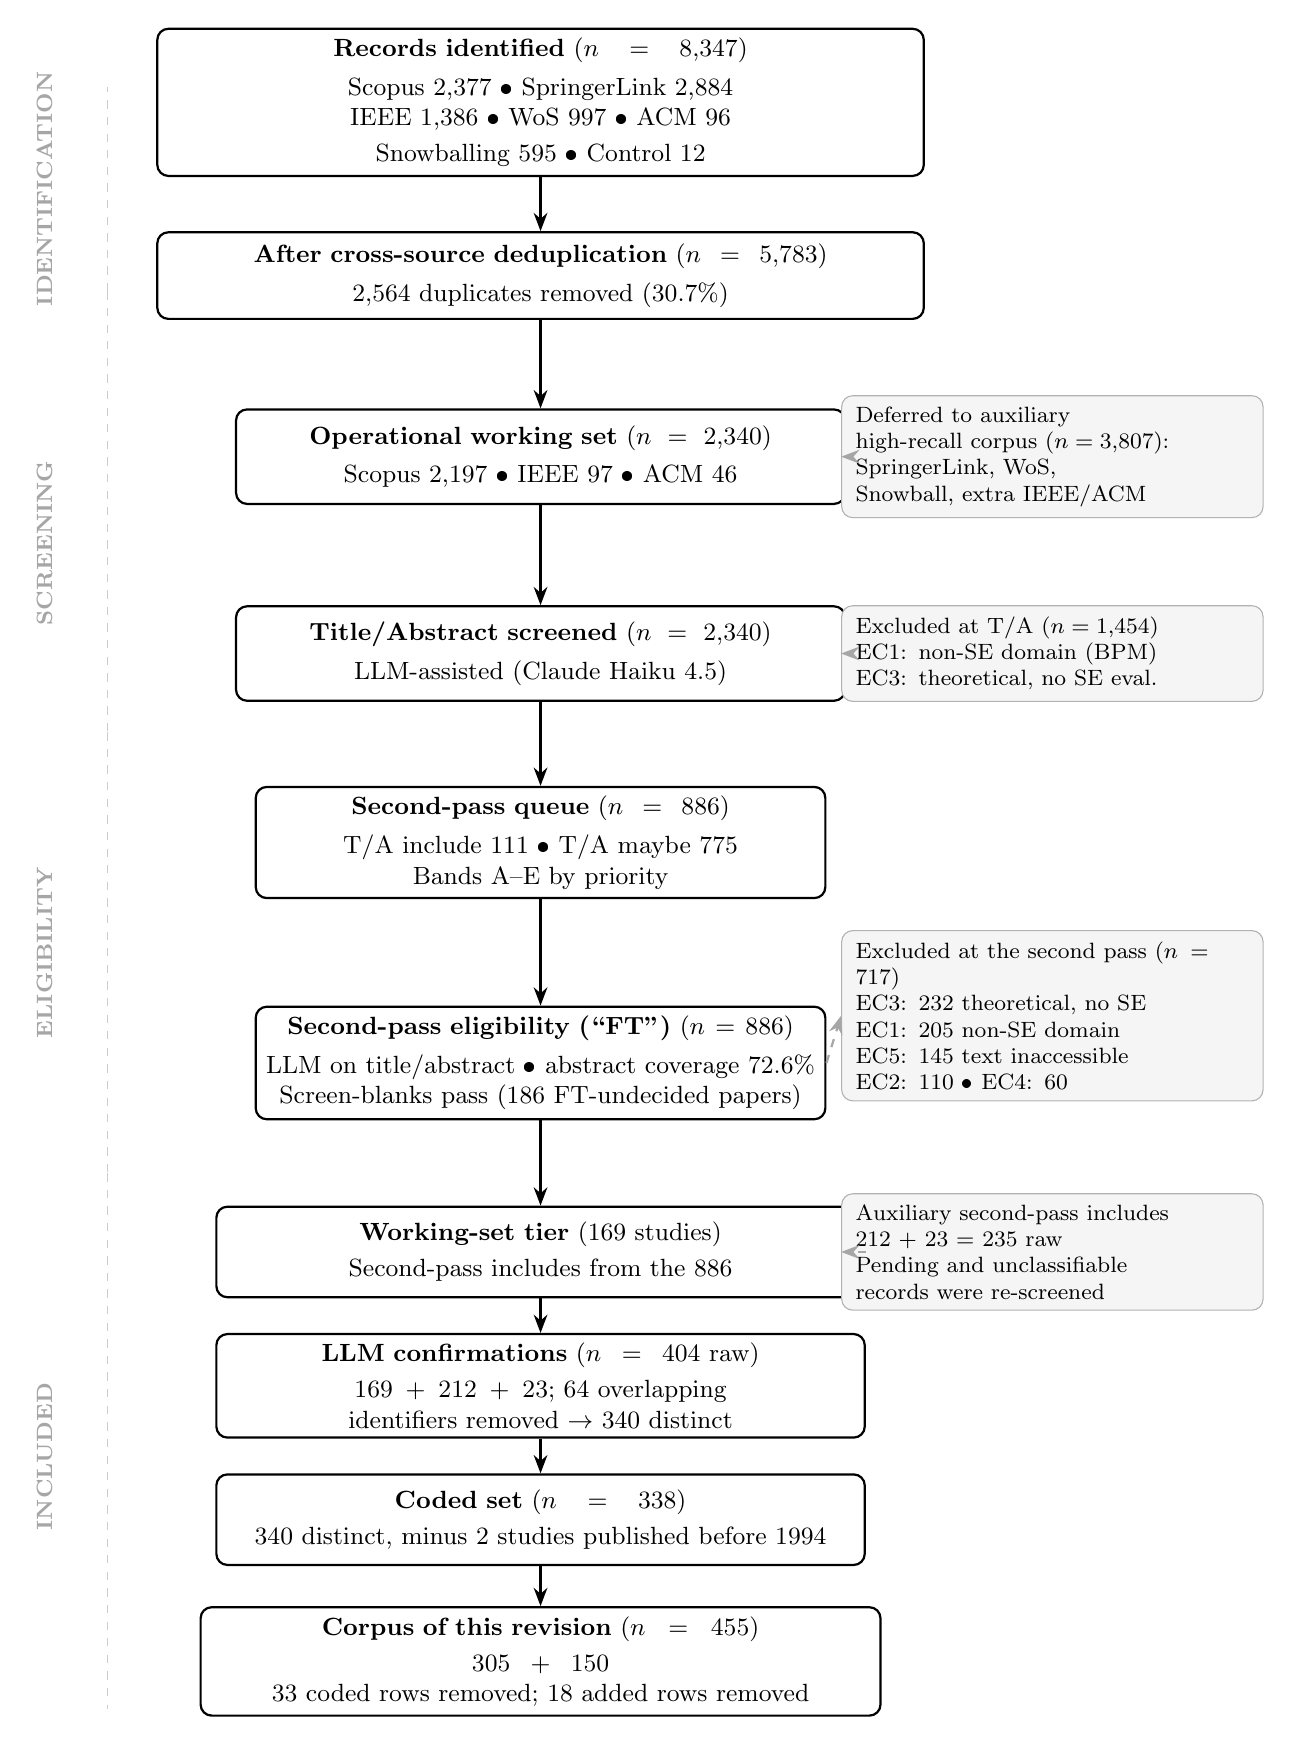
\begin{tikzpicture}[
  %% Main flow boxes (centre column) --- progressively narrower for funnel feel
  stg/.style={draw, rounded corners=4pt, align=center,
              text width=#1, minimum height=1.1cm,
              font=\small, fill=white, thick},
  stg/.default=8cm,
  %% Exclusion / note boxes (right column)
  exc/.style={draw, rounded corners=4pt, align=left,
              inner xsep=5pt, inner ysep=4pt,
              text width=5.0cm, minimum height=0.9cm,
              font=\footnotesize, fill=gray!8, draw=gray!60},
  %% Phase labels (left column)
  lbl/.style={font=\footnotesize\bfseries, text=gray!70,
              rotate=90, anchor=center},
  arr/.style={->, >=Stealth, thick},
  sidearr/.style={->, >=Stealth, dashed, draw=gray!70, thick},
]

%% -- PHASE: IDENTIFICATION ----------------------------------------------

\node[lbl] at (-6.8,-1.1) {IDENTIFICATION};
\draw[gray!40, dashed] (-6.0,-2.4) -- (-6.0, 0.2);

\node[stg=9.5cm, minimum height=1.3cm] (id) at (-0.5,0)
  {\textbf{Records identified} ($n = 8{,}347$)\\[3pt]
   Scopus~2{,}377 \textbullet{} \mbox{SpringerLink}~2{,}884\\
   IEEE~1{,}386 \textbullet{} WoS~997 \textbullet{} ACM~96\\[2pt]
   Snowballing~595 \textbullet{} Control~12};

\node[stg=9.5cm] (dedup) at (-0.5,-2.2)
  {\textbf{After cross-source deduplication} ($n = 5{,}783$)\\[3pt]
   2{,}564 duplicates removed (30.7\%)};

\draw[arr] (id) -- (dedup);

%% -- PHASE: SCREENING ----------------------------------------------------

\node[lbl] at (-6.8,-5.6) {SCREENING};
\draw[gray!40, dashed] (-6.0,-2.4) -- (-6.0,-8.0);

\node[stg=7.5cm, minimum height=1.2cm] (ws) at (-0.5,-4.5)
  {\textbf{Operational working set} ($n = 2{,}340$)\\[3pt]
   Scopus~2{,}197 \textbullet{} IEEE~97 \textbullet{} ACM~46};

\node[exc] (wsdrop) at (6.0,-4.5)
  {Deferred to auxiliary\\high-recall corpus ($n = 3{,}807$):\\
   \mbox{SpringerLink}, WoS,\\Snowball, extra IEEE/ACM};

\draw[arr] (dedup) -- (ws);
\draw[sidearr] (ws.east) -- (wsdrop.west);

\node[stg=7.5cm, minimum height=1.2cm] (ta) at (-0.5,-7.0)
  {\textbf{Title/Abstract screened} ($n = 2{,}340$)\\[3pt]
   LLM-assisted (Claude Haiku 4.5)};

\node[exc] (taexc) at (6.0,-7.0)
  {Excluded at T/A ($n = 1{,}454$)\\
   EC1: non-SE domain (BPM)\\
   EC3: theoretical, no SE eval.};

\draw[arr] (ws) -- (ta);
\draw[sidearr] (ta.east) -- (taexc.west);

%% -- PHASE: ELIGIBILITY --------------------------------------------------

\node[lbl] at (-6.8,-10.8) {ELIGIBILITY};
\draw[gray!40, dashed] (-6.0,-8.0) -- (-6.0,-13.6);

\node[stg=7cm, minimum height=1.3cm] (ftq) at (-0.5,-9.4)
  {\textbf{Second-pass queue} ($n = 886$)\\[3pt]
   T/A include~111 \textbullet{} T/A maybe~775\\
   Bands~A--E by priority};

\draw[arr] (ta) -- (ftq);

\node[stg=7cm, minimum height=1.4cm] (ft) at (-0.5,-12.2)
  {\textbf{Second-pass eligibility (``FT'')} ($n = 886$)\\[3pt]
   LLM on title/abstract \textbullet{} abstract coverage 72.6\%\\
   Screen-blanks pass (186 FT-undecided papers)};

\node[exc] (ftexc) at (6.0,-11.6)
  {Excluded at the second pass ($n = 717$)\\
   EC3: 232 theoretical, no SE\\
   EC1: 205 non-SE domain\\
   EC5: 145 text inaccessible\\
   EC2: 110 \textbullet{} EC4: 60};

\draw[arr] (ftq) -- (ft);
\draw[sidearr] (ft.east) -- (ftexc.west);

%% -- PHASE: INCLUDED ----------------------------------------------------

\node[lbl] at (-6.8,-17.2) {INCLUDED};
\draw[gray!40, dashed] (-6.0,-13.6) -- (-6.0,-20.4);

\node[stg=8cm, minimum height=1.15cm] (wsinc) at (-0.5,-14.6)
  {\textbf{Working-set tier} (169 studies)\\[2pt]
   Second-pass includes from the 886};

\node[exc] (auxinc) at (6.0,-14.6)
  {Auxiliary second-pass includes\\
   212 + 23 = 235 raw\\
   Pending and unclassifiable\\
   records were re-screened};

\draw[arr] (ft) -- (wsinc);
\draw[sidearr] (wsinc.east) -- (auxinc.west);

\node[stg=8cm, minimum height=1.15cm] (raw) at (-0.5,-16.3)
  {\textbf{LLM confirmations} ($n = 404$ raw)\\[2pt]
   $169 + 212 + 23$; 64 overlapping identifiers removed $\rightarrow$ 340 distinct};

\draw[arr] (wsinc) -- (raw);

\node[stg=8cm, minimum height=1.15cm] (coded) at (-0.5,-18.0)
  {\textbf{Coded set} ($n = 338$)\\[2pt]
   340 distinct, minus 2 studies published before 1994};

\draw[arr] (raw) -- (coded);

\node[stg=8.4cm, minimum height=1.25cm] (inc) at (-0.5,-19.8)
  {\textbf{Corpus of this revision} ($n = 455$)\\[2pt]
   $305 + 150$\\
   33 coded rows removed; 18 added rows removed};

\draw[arr] (coded) -- (inc);

\end{tikzpicture}
\caption{PRISMA 2020 flow of the study selection. The 2{,}340 and the
  3{,}807 are identifier lists. They share 364 papers, and their union is
  the 5{,}783. The included phase
  continues through the auxiliary screen, the removal of overlapping
  identifiers, the removal of two pre-1994 studies, and the human re-screen.
  The mapped set is 455 studies (Table~\ref{tab:ledger}). The 318-study
joint tables are an older cut (381 records minus 63 duplicates) and are
not a node of this flow. In the original run, 595 records with no abstract
and 16 records that stayed pending were closed under EC5; this revision
re-screened those records.}
\label{fig:prisma}
\end{figure}


\section{Results and Synthesis}
\label{sec:slr-synthesis}

\subsection{Overview of Included Studies}

This revision includes \textbf{455 studies}: 305 that remain from the
coded list of 338, plus 150 that remain after the eligibility pass.

The 338 are the LLM list of 340 studies, minus two papers from 1991 and
1992. The human re-screen marked 188 records as eligible. Twenty of them
repeated a study already in the list, leaving 168. Eighteen of those 168
fail an inclusion or exclusion rule and are removed. Seventeen had been
read from an abstract or a PDF: the extraction either names no technique
in IC4a--IC4d, or the text is outside software development (EC1 or EC2).
One, identifier \texttt{46815264}, is dated 1992 and fails IC1. Forty-six
others had been labelled ``none of the four'' even though the extraction
names a technique; they stay, with that family. The 18 removals and the
46 assignments are listed in \texttt{corpus\_eligibility\_pass.csv}. Of the
150 that remain, 11 were read as a PDF, 63 from the abstract, and 76 from
the title only.

Thirty-three studies, 33 of the 338 coded includes (9.8\%), are then
removed. The re-screen sheets do not mark them: on all 4{,}005 rows the
decision equals the suggestion. The list was rebuilt from the title or
abstract the LLM treated as sufficient. Each was an include for which
that text does not support inclusion. The object is generic
process mining or forecasting, a business process, product execution, or
system architecture. Two of them, \texttt{96767878} and \texttt{f449ac41},
have no abstract, and the inclusion note itself asks for the full text.
Seventeen come from the working set, seven from the first auxiliary tier,
and nine from the second. The list is
\texttt{labels\_ta\_insufficient\_for\_include.csv}. The coded studies that
remain are 305, and the corpus is $305 + 150 = 455$.

The three technique families were marked on \textbf{379} of the 455: the
305, plus the 74 added studies that had an abstract or a PDF and meet at
least one content criterion. One of those 379, PRIMAD, has all three
families. The 76 studies known only by the title were left blank. A blank
is not counted as a no.

Table~\ref{tab:ledger} is the single count of every cut used in the
paper. Four of those rows answer different questions, and they are not
interchangeable. The context set is the 455. The 33 removed from the
coded list are the LLM includes whose title or abstract does not support
inclusion. The 74 added studies stay because the extraction names a
technique in IC4a--IC4d. The 76 title-only studies were not marked, and a
blank is not treated as satisfying a content criterion. The rows with
technique-family codes filled before this round were the 338; 305 remain
after the removal of 33. The rows with at least one family mark, including
the 74 added studies, are the 379. The intersection of process mining, a
stochastic model, and forecasting is one study inside that 379.
Each research question is answered on the cut named in its sentence. The
working-set family codes use 150 studies. That is the 169 extraction minus
17 studies whose title or abstract does not support inclusion, and minus
two extra identifiers of one paper the corpus keeps once
(\texttt{2647ea07}). The joint family codes use 292 studies. That is the
318 minus those 17, minus seven studies from the first auxiliary tier
removed for the same reason, and minus the two pre-1994 papers. Nine of
the 33 removed studies are not in the 318.
The joint tables use 318. That 318 is what remained after 63 duplicate
records were removed from an earlier combined list of 381. The 340 is what
remained after 64 duplicate records were removed from 404 raw
confirmations. The two cuts were built by different removals. Adding the
23 studies of the second auxiliary pass to 318 does not produce 340. The
33 removed above are the coded includes whose title or abstract does not
support inclusion. The appendix lists the 455 studies and groups them by
family.

\begin{table}[htbp]
\centering
\caption{Counts used in this paper. Each row is a different cut.}
\label{tab:ledger}
\small
\begin{tabular}{lp{8.1cm}}
\toprule
\textbf{Studies} & \textbf{Meaning} \\
\midrule
8{,}347 & Records retrieved, before deduplication. \\
5{,}783 & Records after deduplication. \\
2{,}340 & Working-set identifier list. 1{,}976 of these identifiers are in the 5{,}783. \\
3{,}807 & The other identifiers in the 5{,}783 ($5{,}783-1{,}976$). This list holds the second identifier of 364 papers that are also in the working set. The union is 5{,}783. \\
404 & Raw LLM confirmations (169 + 212 + 23). \\
340 & Distinct LLM list (404 minus 64 duplicate records). \\
338 & The 340 minus two papers from 1991 and 1992. \\
381 & Earlier combined list, before the 318 cut. \\
318 & Joint tables (381 minus 63 duplicate records). Not 340 minus 23. \\
150 & Working-set family codes. The 169 minus 17 removed studies and minus 2 extra identifiers of one paper. \\
292 & Joint family codes. The 318 minus 24 removed studies and minus 2 pre-1994 papers. \\
33 & Coded includes removed (33 of 338, 9.8\%). The title or abstract does not support inclusion. Not marked on the 4{,}005-row sheets. \\
305 & Coded studies that remain (338 minus 33). \\
455 & This revision (305 + 150). Of 168 after de-duplication, 18 were also removed. \\
379 & At least one family mark (305 + 74). Not a rate over the 455. \\
76 & Added studies known only by the title. Marks left blank. \\
\bottomrule
\end{tabular}
\end{table}

The list is \texttt{included\_studies\_506.csv} (455 rows; the filename
keeps an earlier count). The file of 340 rows is kept so the removal of
the two pre-1994 papers can be checked. Thirty-five of the 150 added
studies were assigned a model score of at least 4/8. A score taken from an
abstract is not a quality assessment of the study, and no score is used to
keep or drop a study. F2 and F5 are withdrawn, and their percentages are
not reported. The percentages under F1, F3, and F4, apart from the count
of one study in 379, are the family codes on the 150 and the 292. On the
original 169, TF-PM with neither TF-ST nor TF-FC is 105, not 68: the 68
are the code that is exactly TF-PM, and 37 more are TF-PM with TF-MSR
only. On the original 318 the same definition is 138, not 78: the 78 are
TF-ST together with TF-FC and no TF-PM. The figures below use the 150 and
the 292. Their status is stated once in Section~\ref{sec:slr-gaps}.

The 150 working-set studies that remain span 1995--2026 (publications dated 2026
that were already indexed on 12~April~2026 are retained), with a clear
acceleration from 2014 onward (Figure~\ref{fig:year-dist}). One hundred
and four of them (69.3\%) appeared in 2015--2026.
A completed SEGRESS~\cite{kitchenham2023segress} reporting checklist is in
Appendix~\ref{app:segress}.

\begin{figure}[htbp]
\centering
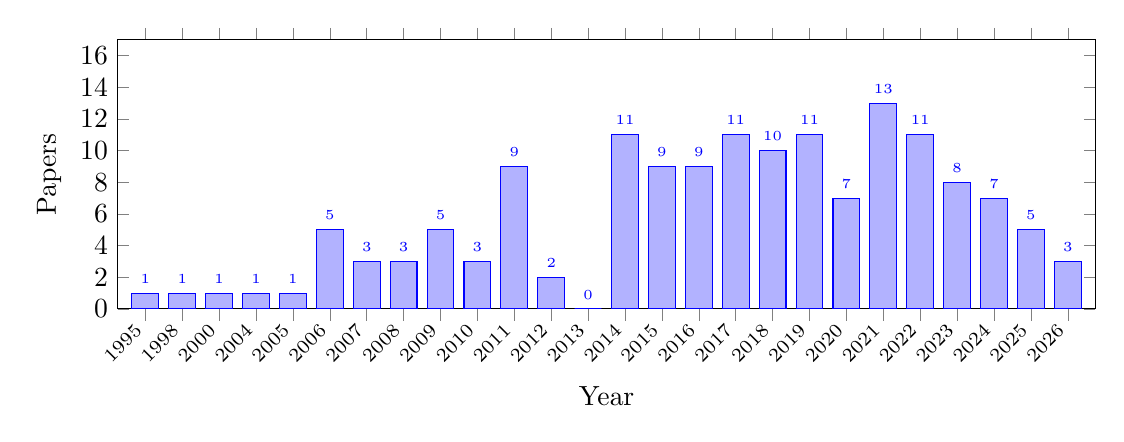
\begin{tikzpicture}
\begin{axis}[
  ybar,
  bar width=0.34cm,
  width=14cm, height=5cm,
  xlabel={Year},
  ylabel={Papers},
  xtick=data,
  xticklabels={1995,1998,2000,2004,2005,2006,2007,2008,2009,2010,2011,2012,2013,2014,2015,2016,2017,2018,2019,2020,2021,2022,2023,2024,2025,2026},
  x tick label style={rotate=45, anchor=east, font=\scriptsize},
  ymin=0, ymax=17,
  ytick={0,2,4,6,8,10,12,14,16},
  enlarge x limits=0.03,
  fill=gray!40,
  draw=black,
  nodes near coords,
  nodes near coords style={font=\tiny, above},
]
\addplot coordinates {
  (1,1)(2,1)(3,1)(4,1)(5,1)(6,5)(7,3)(8,3)(9,5)(10,3)(11,9)(12,2)(13,0)(14,11)(15,9)(16,9)(17,11)(18,10)(19,11)(20,7)(21,13)(22,11)(23,8)(24,7)(25,5)(26,3)
};
\end{axis}
\end{tikzpicture}
\caption{Publication year of the 150 working-set studies that remain.}
\label{fig:year-dist}
\end{figure}

By document type, the majority are conference papers and journal articles.
By source database, Scopus is the dominant contributor, followed by
IEEE~Xplore and ACM~DL. Data extraction was completed for all 169 studies
using a structured LLM-assisted pipeline (\textit{claude-haiku-4-5-20251001})
operating on locally available PDFs (75/169, of which 73 were operationally
coded in the triangulation subset) or abstract/title metadata (94/169).

\subsection{Inclusion Criterion Coverage}

Figure~\ref{fig:ic-dist} shows the distribution of inclusion criteria among
the 150 working-set studies that remain (criteria are non-exclusive; a paper may satisfy
multiple).

\begin{figure}[htbp]
\centering
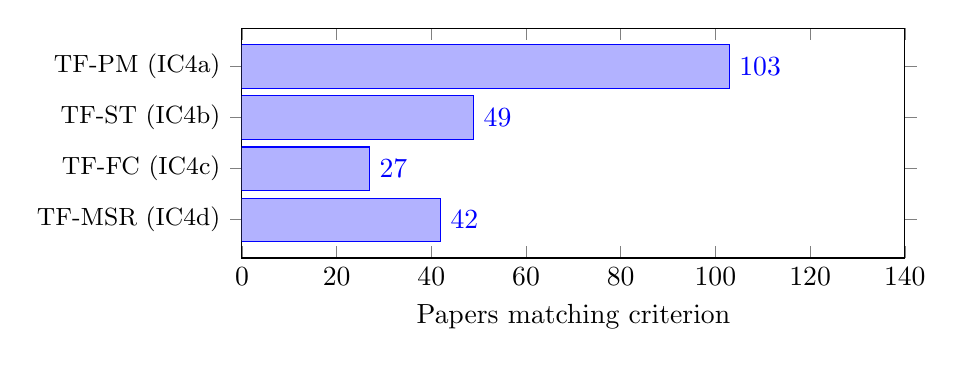
\begin{tikzpicture}
\begin{axis}[
  xbar,
  bar width=0.55cm,
  width=10cm, height=4.5cm,
  xlabel={Papers matching criterion},
  symbolic y coords={TF-MSR (IC4d), TF-FC (IC4c), TF-ST (IC4b), TF-PM (IC4a)},
  ytick=data,
  y tick label style={font=\small},
  xmin=0, xmax=140,
  nodes near coords,
  nodes near coords align={horizontal},
  fill=gray!40,
  draw=black,
  enlarge y limits=0.25,
]
\addplot coordinates {
  (103,{TF-PM (IC4a)})
  (49,{TF-ST (IC4b)})
  (27,{TF-FC (IC4c)})
  (42,{TF-MSR (IC4d)})
};
\end{axis}
\end{tikzpicture}
\caption{Inclusion criteria matched by the 150 working-set studies that remain. Counts
are non-exclusive. TF-PM, TF-ST, TF-FC, and TF-MSR are the content criteria
IC4a--IC4d. TF-PM with neither TF-ST nor TF-FC is 91 of these 150.}
\label{fig:ic-dist}
\end{figure}

TF-PM (process mining applied to SE artifacts) is the dominant criterion,
matched by 103 papers (68.7\%). TF-MSR (repository mining for process modeling)
is second at 42 papers (28.0\%). TF-ST (stochastic modeling) appears in 49
papers (32.7\%) and TF-FC (forecasting of process metrics) in 27 papers
(18.0\%). TF-PM with neither TF-ST nor TF-FC is 91 papers (60.7\%). The
other 101 of the 150 do not carry TF-ST, and $49+101=150$. That split is
the stored family-code count labeled F1 in Section~\ref{sec:slr-gaps}.

\subsection{Prevalent Exclusion Patterns}

Among the 717 FT-excluded papers (Table~\ref{tab:ft-screening}), the largest
exclusion reason is EC3 (algorithmic or theoretical contribution without
software-engineering evaluation, $n=232$), indicating a substantial body of
process mining and stochastic modeling research that has not been empirically
applied to software engineering contexts. EC1 (domain exclusively outside
software development, $n=205$) is the second-largest reason and consists
primarily of generic business process management (BPM) studies that use the
same terminology as the search strings but apply techniques to organizational
processes unrelated to SDLC. EC5 (full text inaccessible, active post-audit
$n=145$; original historical stratum $n=148$) closes the group of large
strata, followed by EC2 (software as implementation platform
rather than analyzed process, $n=110$) and EC4 (out-of-scope secondary study,
$n=60$). EC counts are non-exclusive: the sum of per-EC counts
($232+205+145+110+60 = 752$) exceeds the 717 excluded papers by 35,
corresponding to papers that triggered more than one EC simultaneously. EC3
and EC1 are the two largest reasons in this exclusion list. That is a
property of the list. It does not confirm the family codes in
Section~\ref{sec:slr-gaps}.

\subsection{Full-Text Extraction and PDF-Based Triangulation}
\label{sec:slr-pdf-enrichment}

Structured data extraction was performed on the full 169-study set using the
extraction template defined in Table~\ref{tab:extraction}. For each study,
the LLM extracted the research question, study type, research contribution,
PM technique, stochastic technique, software artifact, software process, data
source, dataset availability, tool used, main finding, limitations, and
replication-package status. Title-and-abstract metadata was used as the
primary input for studies without locally available PDFs (94/169); for the
remaining 75/169 studies a locally accessible PDF was available and used to
triangulate against the LLM-extracted fields. Of these 75 PDFs, 73 were
fully coded in the operational triangulation spreadsheet used for the
figures and positioning tables below.

The 73-paper PDF triangulation subset is therefore not a separate selection
stage and does not override the PRISMA counts. It does not confirm the
fields behind F1--F5. On 31 studies the exact match between a human rater
and the model on the free-text fields is 0\%. F1, F3, and F4 were not
re-marked in this revision.

Figure~\ref{fig:pdf-decision-dist} summarizes the operational triage profile
of the 73 coded PDFs (54 confirm-include, 13 confirm-include with
caveats, 6 confirm-exclude after full-text inspection); the formal selection
decisions reported in the PRISMA flow (Figure~\ref{fig:prisma}) are
unchanged.

\begin{figure}[tbp]
\centering
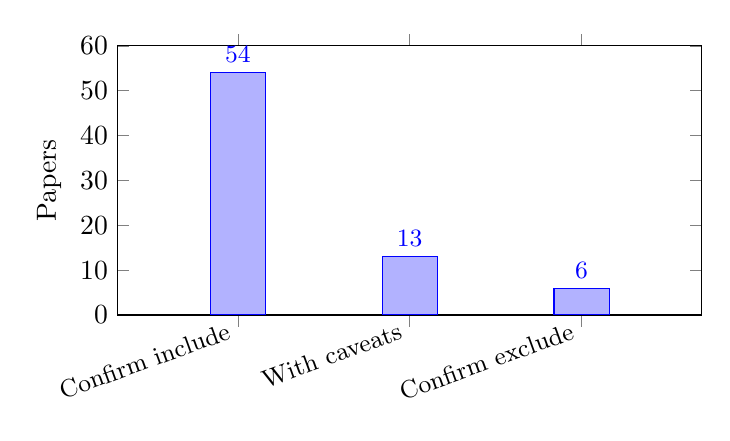
\begin{tikzpicture}
\begin{axis}[
  ybar,
  bar width=0.7cm,
  width=9cm, height=5cm,
  ylabel={Papers},
  symbolic x coords={Confirm include,With caveats,Confirm exclude},
  xtick=data,
  x tick label style={font=\small, rotate=20, anchor=east},
  ymin=0, ymax=60,
  ytick={0,10,20,30,40,50,60},
  nodes near coords,
  nodes near coords style={font=\small, above},
  fill=gray!45,
  draw=black,
  enlarge x limits=0.35,
]
\addplot coordinates {(Confirm include,54) (With caveats,13) (Confirm exclude,6)};
\end{axis}
\end{tikzpicture}
\caption{Reading of the 73 PDFs: 54 confirm-include, 13 confirm-include with
caveats, and 6 confirm-exclude. These labels are not the screen decisions
Include, Maybe, and Exclude. The PRISMA flow is unchanged.}
\label{fig:pdf-decision-dist}
\end{figure}

\subsection{RQ1: Application Landscape}
\label{sec:slr-rq1}

\subsubsection{RQ1.1: SDLC Phases Covered}

The phase field on the 169 extraction was not recomputed after 17 studies
and two extra identifiers left that cut. Those phase percentages are not
reported. The family codes that are reported use the 150 studies that
remain. They are not a description of the 455.

The phase field was not re-marked.

\subsubsection{RQ1.2: Event Log Sources and Construction}

The source families, the public-dataset count, and the replication-package
count are free-text fields. On 31 studies the exact match between a human
rater and the model on those fields is 0\%, and the fields were not
re-extracted. F2 is withdrawn. Those percentages are not reported, and
they do not motivate RA1.

A complementary body of work constructs Markov models directly from GitHub
repository traces, bypassing explicit process discovery in favour of manual
state-space definition. Jo et al.\ \cite{jo2023} modelled developer activities
in GitHub repositories as Discrete-Time Markov Chains (DTMCs), finding that
commits account for 62.73\% of long-term activity, and employed probabilistic
temporal logic to extract collaboration patterns relevant to project management.
This approach was extended in \cite{jo2024}, where Probabilistic Model Checking
with Computation Tree Logic was applied across five repositories to characterise
temporal dynamics, state-transition probabilities, and key behavioural drivers,
yielding transparent and explainable project forecasts. Ortu et al.\ \cite{ortu2023}
complemented these structural analyses by combining Markov chains with social
network analysis to identify fault-insertion and fault-fixing behavioural patterns
across Apache Software Foundation projects, demonstrating that developer expertise
significantly moderates defect introduction likelihood. Collectively, these studies
confirm that SDLC event logs extracted from public repositories are sufficiently
rich to support state-transition modelling. However, the event-to-state mapping
adopted across these works is defined manually and differs from study to study;
none derives the state space from a discovered process model.


\subsection{RQ2: Techniques and Prediction}
\label{sec:slr-rq2}

\subsubsection{RQ2.1: Discovery Algorithms Applied to SDLC}

The canonical origin of process mining applied to software development contexts
can be traced directly to the foundational contributions of Cook and Wolf in the
mid-1990s. In their seminal work, \cite{cook1995} introduced three automated
process discovery methods---algorithmic grammar inference, Markov models, and
neural networks---demonstrating that finite-state machine representations of
software processes could be extracted automatically from event traces,
substantially lowering the barrier to formal process modeling. This line of
inquiry was consolidated in \cite{cook1998}, which refined the event-based
discovery methodology and established the conceptual vocabulary of inferring
workflow structures from historical execution data, a paradigm that remains
central to the field today. Notably, both contributions embedded stochastic
reasoning---particularly Markov chain representations---within the discovery
pipeline, anticipating the probabilistic extensions that would later characterise
mature process mining frameworks. The translation of these principles into an
explicit, named framework for software engineering contexts was accomplished by
\cite{rubin2007}, who applied the ProM toolkit to source code management logs
and demonstrated multi-perspective analysis spanning control-flow, informational,
and organisational dimensions. Together, these three works constitute the seminal
arc of TF-PM, establishing automated discovery from SDLC event logs as both
technically feasible and analytically productive.

The family-code count on the 150 working-set studies that remain, which
this revision did not re-mark, has 103 studies (68.7\%) matching TF-PM.
The same count has 27 papers (18.0\%) matching TF-FC.
The names of individual algorithms are free-text
fields. They were not re-extracted. Those names are not reported.

TF-ST is 49 of these 150 (32.7\%). The other 101 do not carry that code,
and $49+101=150$. The column \texttt{stochastic\_technique} is not that
code. On these 150 rows it is \texttt{none} for 96 and a named technique
for 54, and $96+54=150$. Twenty-six of the 54 also contain the token
\texttt{other}. Six rows coded TF-ST have \texttt{none} in the column, and
11 rows with a named technique are not coded TF-ST. On the original 169
the same column was \texttt{none} for 110 rows, and 29 rows also contained
\texttt{other}. Set beside TF-ST $=52$, those two figures do not partition
169: $52+110=162$ and $110+29+52=191$. The four technique bars in
Figure~\ref{fig:pdf-technique-dist} are tokens in that column. They are
not a partition of the 49.

\begin{figure}[tbp]
\centering
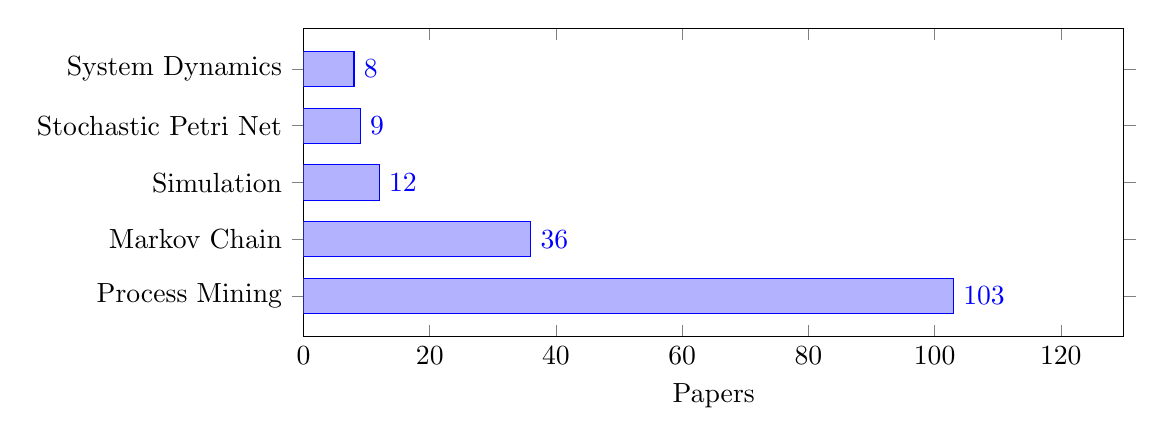
\begin{tikzpicture}
\begin{axis}[
  xbar,
  bar width=0.45cm,
  width=12cm, height=5.5cm,
  xlabel={Papers},
  symbolic y coords={Process Mining,Markov Chain,Simulation,Stochastic Petri Net,System Dynamics},
  ytick=data,
  xmin=0, xmax=130,
  nodes near coords,
  nodes near coords align={horizontal},
  fill=gray!45,
  draw=black,
  enlarge y limits=0.18,
]
\addplot coordinates {
  (103,{Process Mining})
  (36,{Markov Chain})
  (12,{Simulation})
  (9,{Stochastic Petri Net})
  (8,{System Dynamics})
};
\end{axis}
\end{tikzpicture}
\caption{Process mining is the TF-PM family code on the 150 working-set
studies that remain. The other four bars are tokens in
\texttt{stochastic\_technique}. They are not a partition of TF-ST, and a
paper may carry more than one token. These counts were not re-marked.}
\label{fig:pdf-technique-dist}
\end{figure}

\subsubsection{RQ2.2: Predictive and Stochastic Techniques}

Three distinct sub-families of stochastic techniques emerge from the confirmed
literature. The first, \textbf{Markov-chain-based prediction}, encompasses
models that represent software processes as discrete state transitions, including
reinforcement learning agents grounded in Markov Decision Processes for
pull-request outcome prediction \cite{joshi2024}, probabilistic risk
quantification from repository data \cite{jeon2015}, defect removal
effectiveness under code churn \cite{tian2005}, agile state-space planning and
tracking \cite{tyagi2021}, release-time forecasting via generalised reliability
models \cite{washizaki2015}, and Stochastic Automata Networks for Waterfall team
estimation \cite{massitela2018}. The second sub-family, \textbf{stochastic
Petri nets}, models concurrency and asynchrony in DevOps and CI/CD pipelines
through non-Markovian specifications \cite{benmesmia2021} and sensitivity
analyses that identify bottleneck stages governing delivery probability
\cite{bhadra2022,bhadra2023}. The third sub-family, \textbf{Monte Carlo
simulation}, drives project-level forecasting in hybrid System Dynamics models
\cite{li2020}, agile risk assessment frameworks \cite{lunesu2021}, cycle-time
economic analysis \cite{magennis2015}, and the PRIMAD digital-twin architecture
for SDLC \cite{guinea2025}.

Despite their methodological diversity, the cited descriptions share a
parametrisation pattern. Transition
probabilities, firing rates, and distributional parameters in these
descriptions come from aggregate project statistics---historical defect
counts, phase-level duration averages, or summary velocity metrics---rather
than from transition frequencies extracted through process mining of
fine-grained event logs \cite{nafreen2020,bhadra2022,li2020}. In the same
descriptions, model states stay anchored to coarse lifecycle phases. This
is a reading of those descriptions. It is not a re-mark of the family codes
labeled F3, which are the counts on the 150 and the 292.

Three studies exemplify the productive convergence of process mining and
stochastic modelling at the component level. Incerto~\cite{incerto2025}
demonstrated that variable-length Markov chains outperform eighteen existing
stochastic conformance-checking techniques across ten of eleven benchmark
datasets, establishing that higher-order sequential dependencies in event logs
can be captured without sacrificing computational tractability.
L\'opez-Pintado~\cite{lopezpintado2023} extended process-simulation fidelity by
replacing deterministic resource-availability calendars with probabilistic
counterparts discovered directly from event logs, showing that stochastic
resource representations more accurately replicate empirical cycle-time
distributions. Jalote~\cite{jalote2021} took a complementary perspective,
modelling programmer task sequences as first-order Markov chains derived from
IDE interaction logs and demonstrating that transferring the process patterns of
high-productivity developers to average-productivity peers yields measurable
productivity gains. In the studies cited in this paragraph, the stochastic
layer stays on one analytical concern. That reading does not establish a
unified forecasting pipeline in the literature.

The closest published work to a fully integrated multi-stage architecture is
PRIMAD, proposed by Guinea-Cabrera~\cite{guinea2025}, which orchestrates
pm4py-based process discovery, Akka actor-system simulation, and LightGBM
supervised learning within an evolutionary Digital Twin framework for the SDLC.
Nevertheless, PRIMAD remains at what may be characterised as Level~2 integration:
validation is reported per component rather than across the assembled pipeline,
no formal inter-stage contracts govern the handoffs between discovery,
simulation, and learning modules, and the architecture incorporates no dedicated
Monte Carlo forecasting layer capable of propagating uncertainty estimates
end-to-end. On the family codes filled for the 379 studies, PRIMAD is the
one row that matches the three families. The 338 were not re-marked in this
revision. None of the 74 added studies read from an abstract or a PDF adds
a second triple. The 76 title-only studies are outside that count. A single
code on that cut is not a statement that the literature contains no
end-to-end pipeline.

Studies that combine process mining with forecasting objectives (TF-PM~$\cap$~TF-FC)
tend to approach prediction through \emph{process enhancement} rather than
through explicit stochastic modelling. Gupta~\cite{gupta2017} demonstrated that
combining inductive miner discovery with Markov chain-based predictive analytics
enables identification of recurring failure patterns in software maintenance
workflows. Pourbafrani et al.~\cite{pourbafrani2021} presented SIMPT, a tool
that extracts process trees with time parameters from event logs and enables
interactive what-if simulation; its successor work~\cite{buliga2025} further
integrates generative AI with business process simulation to produce
conformance-preserving what-if scenarios. Caldeira et al.~\cite{caldeira2022}
mine IDE interaction logs and show that process complexity metrics derived from
ProM correlate moderately ($r \approx 0.43$) with software cyclomatic
complexity, achieving predictive accuracies exceeding 92\%, demonstrating the
feasibility of process-derived features for product-quality prediction.

Taken together, the papers cited in this paragraph describe PM output feeding
a downstream model. That reading is not a census of the SE literature. None of
these cited systems is described as reporting a probability distribution
over completion time or remaining steps for an individual process instance.


\subsection{RQ3: Integration and Gaps}
\label{sec:slr-rq3}

\subsubsection{RQ3.1: PM and Stochastic Integration Level}

The family codes on the 150 working-set studies that remain, which this
revision did not re-mark, place rows on the L0--L3 scale defined in
Table~\ref{tab:positioning}: the number of technique families TF-PM, TF-ST,
and TF-FC a study matches. The
largest two-family cluster, comprising papers that touch TF-ST and TF-FC
without TF-PM---including stochastic Petri net models of CI/CD pipelines
\cite{bhadra2022,bhadra2023}, Markov-based project estimation
\cite{massitela2018,tyagi2021}, and Monte Carlo risk simulation
\cite{lunesu2021,magennis2015}---is coded \textbf{L1},
applying stochastic modelling to software processes without any process
discovery layer. Papers spanning TF-PM and TF-ST, such as the VLMC conformance
checker of \cite{incerto2025} and the probabilistic resource-calendar discoverer
of \cite{lopezpintado2023}, are also coded \textbf{L1}: they couple discovered
process structure with stochastic reasoning, but neither closes the loop
toward distributional schedule forecasting. Papers combining TF-PM with TF-FC, such as
\cite{gupta2017} and \cite{caldeira2022}, use process mining descriptively to
assess workflows but lack the stochastic machinery required for Monte Carlo
distributional forecasts. The PRIMAD framework \cite{guinea2025} is the one
triple match in these codes. It assembles event-log discovery,
simulation, and ML prediction, and its evaluation is described as component-wise,
so the code is L2 rather than a validated end-to-end contract. No row
in these 150 codes is \textbf{L3}. L3 would be a row that matches the three
families and states formal interfaces validated end-to-end on SDLC event logs.
These codes do not establish that no such architecture exists in the literature.

The same 150 codes, not a confirmation of a literature pattern, are as follows.
1 of 150 papers (0.7\%) jointly satisfies TF-PM, TF-ST, and TF-FC.
Pairwise codes are TF-PM$\cap$TF-ST in 8 papers (5.3\%), TF-PM$\cap$TF-FC
in 5 papers (3.3\%), and TF-ST$\cap$TF-FC in 18
papers (12.0\%). No row in these 150 codes is an
\textbf{L3} architecture. The same triple on the 292 joint-table studies is also one
paper. A rare code on these cuts is not a rare pattern in the literature.
Figure~\ref{fig:pdf-integration-priority} is the reading priority of the 73
PDFs. It is not the L0--L3 scale of Table~\ref{tab:positioning}.

\begin{figure}[p]
\centering
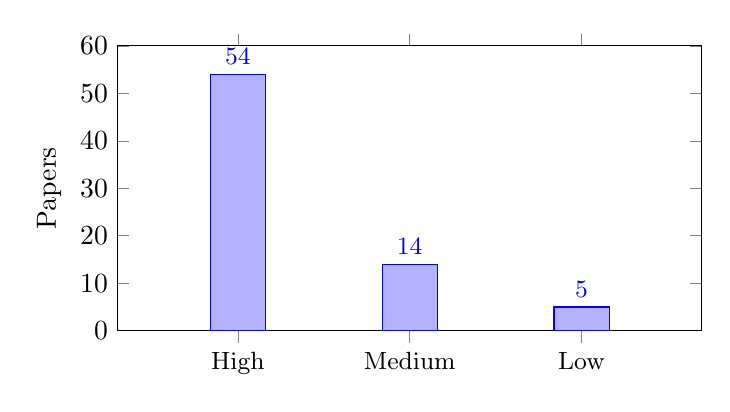
\begin{tikzpicture}
\begin{axis}[
  ybar,
  bar width=0.7cm,
  width=9cm, height=5.2cm,
  ylabel={Papers},
  symbolic x coords={High,Medium,Low},
  xtick=data,
  x tick label style={font=\small},
  ymin=0, ymax=60,
  ytick={0,10,20,30,40,50,60},
  nodes near coords,
  nodes near coords style={font=\small, above},
  fill=gray!45,
  draw=black,
  enlarge x limits=0.35,
]
\addplot coordinates {(High,54) (Medium,14) (Low,5)};
\end{axis}
\end{tikzpicture}
\caption{Reading priority of the 73 PDFs. High, Medium, and Low order those
PDFs for reading. They are not the integration levels L0--L3 in
Table~\ref{tab:positioning} (121, 28, 1, and 0 on the 150 studies).}
\label{fig:pdf-integration-priority}
\end{figure}

\subsubsection{RQ3.2: What the codes do not establish}

Two stored readings of the 150 working-set studies that remain follow.
First, the family-code count labeled F1: 103 papers (68.7\%) match process
mining and 27 (18.0\%) match forecasting of a process metric. TF-PM with
neither TF-ST nor TF-FC is 91 (60.7\%).
Second, the model assigned study types on these 150 rows: 66
(44.0\%) case studies, 29 (19.3\%) tool papers, 26 (17.3\%) theoretical,
12 (8.0\%) simulation-only, 8 (5.3\%) controlled experiments, 5 (3.3\%)
surveys, and 4 (2.7\%) residual categories (mixed, framework, exploratory;
sum: $66+29+26+12+8+5+4 = 150$). That assignment was not re-marked.
F2 is withdrawn: on 31 studies the exact match between a human rater and
the model on the free-text fields is 0\%, so the public-dataset and
replication-package percentages are not reported. The scores in
Table~\ref{tab:qa-results} are what the same model assigned. They do not
stand in for that count.

These readings do not establish that an end-to-end workflow is absent from
the literature. The evidence-type distribution in the 73-PDF subset
(Figure~\ref{fig:pdf-evidence-dist}) is a view of that subset. It is not a
separate selection layer, and it does not confirm the fields.

\begin{figure}[tbp]
\centering
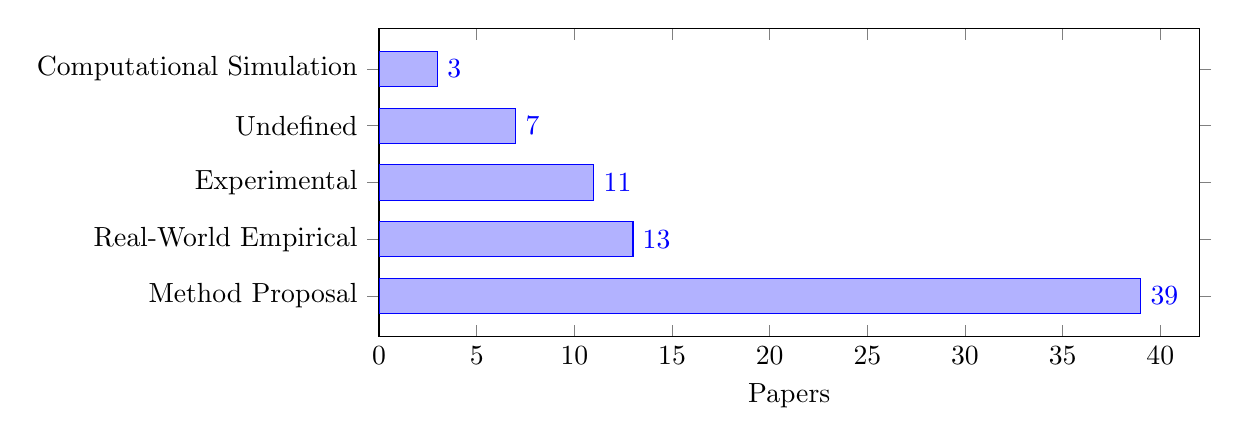
\begin{tikzpicture}
\begin{axis}[
  xbar,
  bar width=0.45cm,
  width=12cm, height=5.5cm,
  xlabel={Papers},
  symbolic y coords={Method Proposal,Real-World Empirical,Experimental,Undefined,Computational Simulation},
  ytick=data,
  xmin=0, xmax=42,
  nodes near coords,
  nodes near coords align={horizontal},
  fill=gray!45,
  draw=black,
  enlarge y limits=0.18,
]
\addplot coordinates {
  (39,{Method Proposal})
  (13,{Real-World Empirical})
  (11,{Experimental})
  (7,{Undefined})
  (3,{Computational Simulation})
};
\end{axis}
\end{tikzpicture}
\caption{Evidence-type distribution in the 73-paper PDF triangulation subset.}
\label{fig:pdf-evidence-dist}
\end{figure}


\section{Discussion}
\label{sec:slr-discussion}

\subsection{Coded counts that are not findings}
\label{sec:slr-gaps}

F2 and F5 are withdrawn. On 31 studies a human rater and the model had
0\% exact agreement on the free-text fields, and those fields were not
re-extracted, so no percentage from them is reported. F1, F3, and F4 are
stored family-code counts. Each sentence names its cut: 150, 292, or the
379 for the triple. None of those percentages is a rate over the 455, none
was re-marked, and none is a finding. None of the five motivates
RA1--RA4.

\begin{description}

\item[F1: Stored family codes on 150 and on 292.]
In the \textbf{working-set cut} (150 papers), 103 (68.7\%) match TF-PM
and 27 (18.0\%) match TF-FC. TF-PM with neither TF-ST nor TF-FC is 91
(60.7\%). In the \textbf{joint cut} (292 papers), 138 (47.3\%) match
TF-PM, 96 (32.9\%) match TF-FC, and 122 (41.8\%) match TF-PM with neither
TF-ST nor TF-FC. The shift between the two cuts is a difference in which
rows the auxiliary corpus added. It is not a claim about the literature.

\item[F2: Withdrawn.]
Event-log construction, dataset availability, and replication-package
status are free-text fields. Exact agreement with a human rater is 0\% on
the 31-study sample, and the fields were not re-extracted. No percentage
is reported. F2 does not motivate RA1. The quality scores are assigned by
the same model. They do not replace this item.

\item[F3: Stored stochastic family codes on 150 and on 292.]
Working-set cut: 49 of 150 papers (32.7\%) match TF-ST, and the other 101
do not ($49+101=150$). TF-ST$\cap$TF-FC covers 18 papers (12.0\%).
TF-PM$\cap$TF-ST covers 8 (5.3\%). Joint cut: 152 of 292 (52.1\%) match
TF-ST, and the other 140 do not ($152+140=292$). TF-ST$\cap$TF-FC covers
80 (27.4\%). TF-PM$\cap$TF-ST covers 10 (3.4\%). The joint cut contains
more rows with TF-ST and without TF-PM than the working-set cut. That is a
difference between the two cuts. It is not a description of the stochastic
literature. The largest second-pass exclusion in the working-set queue is
EC3 (232 of 886). That is a property of this screen. The technique-name
column is not added to these family codes. On the original 169 it does not
partition the rows together with TF-ST, as stated above.

\item[F4: Stored pairwise and triple codes on 150, 292, and 379.]
The family marks
added in this revision are the 74 studies read from an abstract or a PDF
that meet a content criterion, inside the 379. None of those 74 has all
three families. The code file does not record a formal
PM $\rightarrow$ Markov $\rightarrow$ MC $\rightarrow$ ML contract. That
is a property of the file. It is not a finding that no such contract
exists.
Working-set cut (150 papers): the joint convergence
TF-PM$\cap$TF-ST$\cap$TF-FC appears in 1 paper (0.7\%). Pairwise
convergences are TF-PM$\cap$TF-ST: 8 (5.3\%), TF-PM$\cap$TF-FC: 5 (3.3\%),
TF-ST$\cap$TF-FC: 18 (12.0\%). Joint cut (292 papers):
TF-PM$\cap$TF-ST$\cap$TF-FC remains 1 paper (0.3\%), with pairwise
convergences TF-PM$\cap$TF-ST: 10 (3.4\%), TF-PM$\cap$TF-FC: 7 (2.4\%),
TF-ST$\cap$TF-FC: 80 (27.4\%). These counts describe these cuts, not the 455-study corpus. Recall
on the working-set sample is 0.630 (29 of 46; Wilson 95\% CI
0.486--0.755). That figure is not a full-text Recall: a PDF was read
for 0.5\% of the 886 records. The screen missed eligible studies, so a rare pattern in the
338 is not a rare pattern in the literature.
PRIMAD \cite{guinea2025} is that one study inside the 379. It assembles discovery,
simulation, and learning components but validates each independently and
leaves the unified pipeline unevaluated. Its scope is SDLC-oriented: it builds a
digital twin from issue-tracking flows in JIRA. It combines empirical
process discovery (\texttt{pm4py}), a Python-based simulation core, an Akka
actor system, and supervised machine learning
for context-aware prediction. The reported results are component-wise:
the paper does not validate a coupled PM $\rightarrow$ stochastic
simulation $\rightarrow$ ML pipeline as one architecture.
The 76 added studies read from the title alone are outside this count.

\item[F5: Withdrawn.]
Process-derived features and the coupling of a named mining algorithm with
prediction are free-text fields. On 31 studies the exact match with a
human rater is 0\%, and the fields were not re-extracted. No percentage is
reported, including the share of ML rows that name a process-model
feature. F5 does not motivate RA3. The 19 IC4c title hits from the Scopus
search of 31~October~2026 are reported in Section~\ref{sec:slr-search}.
They are not a substitute for this item.

\end{description}

\subsection{Integration Levels}
\label{sec:slr-positioning}

Table~\ref{tab:positioning} defines the integration levels used throughout
the article and reports their counts. A level is determined only by how many
of the three \emph{technique} families a study matches (TF-PM, TF-ST,
TF-FC); TF-MSR describes the data source and is not counted. With this
single definition, the L1 and L2 rows coincide with the pairwise and triple
intersections reported under F3 and F4.

\begin{table}[htbp]
\centering
\caption{Integration levels of the 150 working-set studies that remain. A level counts
how many of TF-PM, TF-ST, and TF-FC the study matches.}
\label{tab:positioning}
\small
\begin{tabularx}{\linewidth}{@{}c X r X@{}}
\toprule
\textbf{Level} & \textbf{Operational definition} & \textbf{Papers} & \textbf{Example} \\
\midrule
L0 & At most one technique family & 121 & Single-technique studies \\
L1 & Exactly two technique families (TF-PM$\cap$TF-ST: 7;
     TF-PM$\cap$TF-FC: 4; TF-ST$\cap$TF-FC: 17) & 28
   & Incerto~\cite{incerto2025}; L\'opez-Pintado~\cite{lopezpintado2023} \\
L2 & All three technique families (TF-PM$\cap$TF-ST$\cap$TF-FC) & 1
   & PRIMAD~\cite{guinea2025} \\
L3 & All three families coupled through explicit interfaces and validated
     end-to-end & 0 & --- \\
\midrule
\textbf{Total} & & \textbf{150} & \\
\bottomrule
\end{tabularx}

\smallskip
\footnotesize\textit{Note:} L1 counts exclude the single L2 study, so they are
one lower than the inclusive pairwise intersections in F3/F4 (8, 5, 18).
The three exclusive pairs sum to 28 ($7+4+17$).
Figure~\ref{fig:pdf-integration-priority} reports reading priority for 73
PDFs. It is not this L0--L3 scale.
\end{table}

The authors' PATHCAST proposal is one candidate design for L3. It is
\textbf{not} evaluated in this mapping study and is listed only as a
research-agenda hypothesis (RA2--RA4, Section~\ref{sec:slr-agenda}). It
is not inferred from F1--F5.


\subsection{Proposed Taxonomy: SPMF}
\label{sec:slr-taxonomy}

The authors propose the Software Process
Mining and Forecasting (SPMF) taxonomy. It is not inferred from F1--F5.
The three dimensions below are a proposal by the authors:

\begin{description}
\item[Analytical Depth] classifies studies along four levels (labelled AD
  to avoid confusion with the integration levels L0--L3): AD1
  (Descriptive: discovery, conformance), AD2 (Diagnostic: bottleneck, rework),
  AD3 (Predictive: outcome, remaining time), and AD4 (Forecasting:
  distributional, probabilistic).

\item[SDLC Coverage] maps which lifecycle phases are addressed: Requirements
  and Design, Development (coding, commits, PRs), Quality (testing, reviews,
  bugs), Delivery (CI/CD, release), and Operations (incidents, maintenance).

\item[Technique Integration] classifies methodological combination:
  Single (PM only, ML only, MC only), Dual (PM + ML, PM + Markov, Markov + MC),
  and Pipeline (PM $\rightarrow$ Markov $\rightarrow$ MC $\rightarrow$ ML).
\end{description}


\subsection{Research Agenda}
\label{sec:slr-agenda}

The four directions below are proposals by the authors.

\begin{description}
\item[RA1: Standardized Event Log Construction for SDLC.]
  Not inferred from F2. Target: frameworks for transforming
  heterogeneous repository data into comparable event logs with cross-tool
  case correlation.

\item[RA2: Process-Aware Stochastic Forecasting.]
  Not inferred from F3. Target: formal integration of
  mined transition structure with Markov/Monte Carlo forecasting.

\item[RA3: Process-Derived Features for ML.]
  Not inferred from F5. Target: systematic use of conformance, rework,
  and path-entropy features in SE predictors.

\item[RA4: Empirical Benchmarking of Integrated Pipelines.]
  Not inferred from F4. The authors' reading of PRIMAD is reported under
  F4 as a reading of that paper, not as a count of the literature. Target:
  comparable OSS benchmarks with temporal hold-out for end-to-end
  PM--stochastic--ML pipelines. Formal specification and evaluation of
  candidates such as PATHCAST remain future work by the authors.
\end{description}


\subsection{Implications for Practitioners}
\label{sec:slr-practitioners}

No practitioner recommendation is drawn from these counts. The
readings of individual cited papers in Section~\ref{sec:slr-rq2} are
readings of those papers. They are not a recommendation derived from the
169 codes.


\section{Threats to Validity}
\label{sec:slr-threats}

\subsection{Construct Validity}

The search strings may exclude studies that use non-canonical terminology.
This threat is mitigated through three mechanisms: the complementary MSR
string, the frontier stochastic-PM string, and one snowballing iteration
over 595 records attributed to 400 source DOIs
(Section~\ref{sec:slr-search}). The ten control papers were recovered, but
this is a weak check: they were known when the strings were written, so
their recovery does not bound the proportion of relevant studies the
strings miss. Those ten papers are not the snowballing seed list.

\subsection{Internal Validity}

LLM-based screening introduces the risk of systematic decision bias. We
report six aspects of how this risk was handled: (i)~structured outputs;
(ii)~author inspection of \texttt{include} decisions; (iii)~human
validation of the selection against a two-rater reference standard;
(iv)~LLM--LLM cross-model agreement; (v)~the T/A false-positive rate; and
(vi)~the closure rule for unresolved cases used in the original run.

(i)~\textbf{Structured outputs}. All screening responses use a strict JSON
schema, enabling post-hoc analysis of decision patterns and rationale
distributions.

(ii)~\textbf{Author inspection of LLM \texttt{include} decisions}.
Every paper retained at the FT stage of the original run was inspected by the
first author against the PRISMA flow before being added to the 169-study
working-set tier. The escalation set was judged by both reviewers
(Section~\ref{sec:slr-threats}).

(iii)~\textbf{Human validation of the selection}.
\emph{T/A stage.} A stratified random 20\% sample of working-set T/A
decisions ($n=468$) was screened by a human rater blind to the LLM. In the
working set, LLM \texttt{maybe} decisions were forwarded to FT screening
(Section~\ref{sec:slr-results-selection}); against the human labels, the
operational T/A Recall is therefore 72/72 $=1.000$ (Wilson 95\% CI
$0.949$--$1.000$). Counting \texttt{maybe} as a negative, as the R1
manuscript did, gives 18/72 $=0.250$, but that figure describes a decision
rule the working set never applied.

\emph{FT stage --- R1 reference standard withdrawn.} The FT reference
standard reported in R1 ($n=177$) did not record eligibility: all 126 human
\texttt{include} labels coincided with papers for which a PDF had been
obtained, and 50 of the 51 human \texttt{exclude} labels were annotated
``PDF not accessible''. The resulting Recall (0.246) measured PDF
availability, not screening error, and is withdrawn.

\emph{Second pass --- round-2 validation.} The replication files
label this pass FT. Before any new judgement we
pre-registered the check
(\texttt{PREREGISTRATION\_round2\_validation.md}; success if the point
estimate of Recall is at least 0.90). The same 177 records were judged
against Table~\ref{tab:criteria} by two raters, independently, blind to the
LLM and to each other. Disagreements were resolved by consensus. A record
whose text could not be obtained is \texttt{not\_assessable} and leaves the
denominator. Six records are in that class. Agreement between the raters,
before consensus, is $\kappa = 0.654$.

The reference standard is the consensus after a full-text re-reading of the
23 records the first consensus had included and the LLM had excluded. Five of
those 23 are ineligible. One is not assessable, because the file on disk is
a conference programme. Seventeen remain eligible. Against that reference the
LLM's Recall on the working-set sample is 0.630 (29 true positives out of 46 eligible
studies; Wilson 95\% CI 0.486--0.755). This is not a full-text Recall.
A PDF was read for 0.5\% of the 886 records, and the second-pass prompt
received the title and the abstract. Lost evidence is 0.370. MCC is 0.656
and WMCC with false negatives weighted ten to one is 0.168
(Table~\ref{tab:r2-confusion}). The same Recall, 0.630, is obtained if the
second rater's labels are used alone. The first author had computed the
round-1 agreement report on this sample and may remember some LLM decisions.
The second rater had no such exposure. The result is below 0.90, so the
pre-registered rule required a human re-screen of the accessible working-set
records the LLM had excluded.

\emph{Auxiliary tier.} The same rule required a check of LLM non-includes
outside the working set. Three strata were sampled: S1, title/abstract
excludes ($N=2{,}423$, sample 40); S2, full-text excludes ($N=537$, sample
40); S3, records closed without a decision under the extended exclusion rule
($N=611$, sample 60). The first author judged each sampled record. The second
author judged a 30\% subset ($\kappa = 0.494$). Twenty auxiliary includes
were mixed into the sheets so the rater could not infer that every row was
an exclusion. The sample estimates of missed studies are 60.6 in S1, 110.2
in S2, and 12.0 in S3, each already rounded to one decimal. Added before
that rounding they are 182.7. That sample estimator of auxiliary Recall is
0.563 (235 over 235 plus 182.7), which is what triggered the full re-screen.

Both reviewers then screened the working-set exclusions and the rest of
S1, S2, and S3, including the records whose first label was heuristic.
They agreed with 92\% of those suggested labels. The sheets (4{,}005 rows)
store a decision equal to the suggestion on every row, so the labels they
did not accept are not marked there. Rebuilt from the title or abstract
the LLM treated as sufficient, that share of the coded includes is the 33
studies in \texttt{labels\_ta\_insufficient\_for\_include.csv} (33 of 338,
9.8\%), and those 33 are removed from the corpus. The counts of missed
studies below follow the suggested includes. The suggested includes
contain 89 studies the LLM
had missed (10 in the sample, 33 in the rest of S1, 32 in the rest of S2,
14 in the rest of S3). Auxiliary Recall on that count is 0.725 (235 of
324). It is still below 0.90. Seventeen of the 33 S1 includes, and all 14
S3 includes, began as heuristic suggestions. The reviewers' 92\% agreement
covers those suggestions. It does not replace them with a second written
code on each row. After de-duplication, 168 records were new to the list. The eligibility
pass removes 18 of them, so the studies new to the corpus are the 150 in
Section~\ref{sec:slr-synthesis}. The 89 is the auxiliary slice of the
screen. The 150 also includes working-set records the LLM had excluded.

\begin{table}[htbp]
\centering
\caption{Round-2 check of the working-set sample. The human label
is the consensus reference. Lost evidence is $1-\mathrm{Recall}$. The
interval is a Wilson 95\% confidence interval. Six records judged
\texttt{not\_assessable} are outside this table. The Recall in this
table is not a full-text Recall: a PDF was read for 0.5\% of the 886
records, and the prompt received the title and the abstract.}
\label{tab:r2-confusion}
\small
\begin{tabular}{lrrrrccc}
\toprule
 & TP & FP & FN & TN & Recall & 95\% CI & Lost ev. \\
\midrule
Working-set sample & 29 & 5 & 17 & 120 & 0.630 & (0.486, 0.755) & 0.370 \\
\bottomrule
\end{tabular}
\end{table}

The two tables that follow are the round-1 matrices. The row labelled
FT (withdrawn) measured whether a PDF was on disk (Recall 0.246;
$\kappa = 0.122$). That row is withdrawn. The 0.630 above is the Recall
of the working-set sample. It is not a full-text Recall.

\emph{QA and extraction.} On the 31 papers included by both the R1 human
rater and the LLM, LLM QA matched the human rater on 68--100\% per
criterion; free-text extraction fields showed 0\% exact-match agreement.
Those fields were not re-extracted by a human. F2 and F5, which use them,
are withdrawn.

\begin{table}[htbp]
\centering
\caption{Round-1 agreement (Cohen's $\kappa$) between the primary LLM screener (claude-haiku-4-5) and an independent human rater on a stratified random 20\% sample. Interpretation thresholds follow Landis and Koch (1977)~\cite{landiskoch1977}. The T/A row is the title/abstract check. The row ``FT (withdrawn)'' ($\kappa = 0.122$, $n=177$) uses the same PDF-on-disk labels as the withdrawn Recall 0.246. It is not agreement on the criteria, and it is not the $\kappa$ of this revision.}
\label{tab:human-kappa-results}
\begin{tabular}{lccc}
\toprule
Stage & $N$ & $\kappa_{\text{multi}}$ (interpretation) & $\kappa_{\text{binary}}$ (interpretation) \\
\midrule
T/A & 468 & 0.250 (fair) & 0.335 (fair) \\
FT (withdrawn) & 177 & 0.122 (slight) & 0.122 (slight) \\
\bottomrule
\end{tabular}
\end{table}
\begin{table}[htbp]
\centering
\caption{Round-1 human-vs-LLM confusion on a stratified random 20\% sample (human rater as gold standard; counts, not percentages). Recall and Lost Evidence (1$-$Recall) use Wilson 95\% confidence intervals. The T/A row labelled ``maybe$\rightarrow$positive'' treats LLM \texttt{maybe} decisions as positive referrals, matching LLM4SCREENLIT~R6. The row ``FT (withdrawn)'' is not a screening result: Recall 0.246 records whether a PDF was on disk. The Recall of this revision is 0.630 on the working-set sample (Table~\ref{tab:r2-confusion}). That 0.630 is not a full-text Recall.}
\label{tab:human-confusion}
\small
\setlength{\tabcolsep}{3pt}
\begin{tabular}{l rrrr c c c}
\toprule
Stage & TP & FP & FN & TN & Recall & 95\% CI & Lost Ev. \\
\midrule
T/A (strict) & 18 & 4 & 54 & 392 & 0.250 & (0.164, 0.361) & 0.750 \\
T/A (maybe$\rightarrow$pos.) & 72 & 105 & 0 & 291 & 1.000 & (0.949, 1.000) & 0.000 \\
FT (withdrawn) & 31 & 3 & 95 & 48 & 0.246 & (0.179, 0.328) & 0.754 \\
\bottomrule
\end{tabular}
\end{table}

(iv)~\textbf{Cross-model inter-rater agreement (Cohen's $\kappa$)}.
A separate stratified random 20\% sample of T/A ($n_{\text{theoretical}} = 468$ from
the 2{,}340-paper working set) and FT ($n_{\text{theoretical}} = 177$ from
the 886-paper FT queue) decisions was independently re-rated by a second
model from the same provider (\textit{claude-sonnet-4-6}). Of the
468 T/A papers in the sample, 420 produced a parseable decision from the
verifier and entered the agreement computation; the remaining 48 papers
returned a non-parseable response because the abstract was absent, and the
verifier then refused a categorical answer. Those 48 are part of the
verifier workload: 48 of 468 sampled title/abstract papers. They stay out
of $\kappa$ because the verifier returned no category. On the 420
parseable papers the binary observed agreement is 410 of 420. If each of
the 48 is scored as a disagreement, that observed agreement is 410 of 468.
They are not added to Lost Evidence. Lost Evidence is the human
false-negative rate on the pre-registered sample, and these 48 are
verifier responses with no category. The reported $\kappa$ is the
agreement on the 420 papers that produced a parseable decision, out of 468
sampled. All 177 FT
sample papers produced a parseable decision. Both the multi-class
$\kappa$ (over the original \texttt{include}/\texttt{exclude}/\texttt{maybe}
or \texttt{include}/\texttt{exclude}/\texttt{pending} categories) and the
binary $\kappa$ (collapsing the rater outputs to
\texttt{include} versus \texttt{not-include}) are reported in
Table~\ref{tab:kappa-results}. The binary $\kappa$ is reported as a
secondary signal: both binary $\kappa$ values ($0.695$ for T/A and $0.694$
for FT) exceed the substantial-agreement threshold $\kappa \geq 0.61$
\cite{landiskoch1977}, but two LLMs from the same provider may share
systematic biases that inflate LLM--LLM agreement relative to an independent
human check. The multi-class FT $\kappa$ is lower ($0.479$, moderate)
because the verifier returned \texttt{pending} on $25/177$ FT papers where
the primary screener committed to a binary decision.

\begin{table}[htbp]
\centering
\caption{Inter-rater agreement (Cohen's $\kappa$) between primary screener (claude-haiku-4-5) and verifier (claude-sonnet-4-6) on a stratified random 20\% sample. Interpretation thresholds follow Landis and Koch (1977)~\cite{landiskoch1977}.}
\label{tab:kappa-results}
\begin{tabular}{lccccc}
\toprule
Stage & $N$ & $P_o$ & $P_e$ & $\kappa_{\text{multi}}$ (interpretation) & $\kappa_{\text{binary}}$ (interpretation) \\
\midrule
TA & 420 & 82.1\% & 50.2\% & 0.641 (substantial) & 0.695 (substantial) \\
FT & 177 & 76.3\% & 54.5\% & 0.479 (moderate) & 0.694 (substantial) \\
\bottomrule
\end{tabular}
\end{table}

The cross-model verification protocol was also extended to the auxiliary
tier (FT stage, $n = 276$ stratified
random 20\% sample). On the auxiliary tier the verifier (Sonnet 4.6)
returned \texttt{pending} on every paper that the primary screener
(Haiku 4.5) had rated as \texttt{include}, yielding a multi-class
$\kappa = 0.004$ and a binary $\kappa = 0.000$ (Po = 84.8\%). For the
auxiliary-tier T/A stratum ($n=39$), Po = 97.4\% with $\kappa = 0.000$---
a base-rate/prevalence paradox, not evidence of disagreement between raters
when one class dominates. The auxiliary records were afterwards screened by
both reviewers, who agreed with 92\% of the suggested labels
(Section~\ref{sec:slr-threats}). The combined-tier counts still rest on the
family codes of the original coded set, plus the triple-intersection count
on the 379. They were not re-marked in this revision.

\begin{table}[htbp]
\centering
\caption{Auxiliary-tier cross-model agreement (Haiku 4.5 primary vs.\ Sonnet 4.6 verifier). FT: stratified 20\% sample of the 1{,}383 forwarded records. TA: only 39 of the 761 records drawn (20\% of 3{,}806) received a verifier decision, all primary \texttt{exclude}s; that row is not a 20\% sample.}
\label{tab:aux-kappa-results}
\begin{tabular}{lcccccc}
\toprule
Stage & $N$ & $P_o^{\text{multi}}$ & $P_o^{\text{binary}}$ & $\kappa_{\text{multi}}$ & $\kappa_{\text{binary}}$ \\
\midrule
TA & 39 & 97.4\% & 97.4\% & 0.000 (slight) & 0.000 (slight) \\
FT & 276 & 54.3\% & 84.8\% & 0.004 (slight) & 0.000 (slight) \\
\bottomrule
\end{tabular}
\end{table}

(v)~\textbf{T/A false-positive rate}.
The LLM confirmatory pass at FT level (Round~1) rejected 33 of 108 T/A
\texttt{include} papers (30.6\%), primarily for EC3 (algorithm without SE
evaluation). This false-positive rate is consistent with the
T/A-screening false-positive rates reported by Khraisha~et~al.\
\cite{khraisha2024} for medical SLRs (in the 25--35\% range, depending on
domain specificity) and by Syriani~et~al.~\cite{syriani2023} for SE
SLRs. A false positive at title/abstract can be removed at the second
pass. A false negative is not removed by that pass. Recall on
the working-set sample is 0.630. That figure is not a full-text Recall:
a PDF was read for 0.5\% of the 886 records. Missed studies would affect any claim
drawn from the coded rows. This revision draws none from F1--F5. The Round~2
screening reprocessed 495 \texttt{maybe} papers with enriched abstracts and
brought the working-set tier to 169. The corpus of this revision is the
455 in Table~\ref{tab:ledger}.

(vi)~\textbf{Original closure of unresolved uncertainty (revised in resubmission)}.
In the original execution run, papers where metadata remained insufficient or
verifier disagreement could not be resolved were closed under EC5-extended,
biasing toward false negatives. In the working set this rule affected only
records that remained abstract-insufficient at FT; in the auxiliary tier it
closed 611 records (stratum S3), whose share of relevant studies is
estimated in item~(iii). The revised protocol routes
\texttt{maybe}/\texttt{pending} to human review instead
(Section~\ref{sec:slr-llm}).

\subsection{External Validity}

The review is limited to English-language peer-reviewed publications,
which leaves out work in other languages.
The broad time span (January 1994 to 12~April~2026) and five-database
coverage mitigate geographic and temporal bias. Grey literature is
excluded. The stop rule is the document type at search time: journal
articles, conference papers, and workshop papers. Theses, preprints, and
technical reports were not searched in a separate round. The auxiliary
identifier list (3{,}807 rows; Section~\ref{sec:slr-results-selection})
was screened in full. It shares 364 papers with the working set.
The mapped set is the 455 in
Table~\ref{tab:ledger}. The working set was built from Scopus, IEEE, and
ACM. SpringerLink, Web of Science, and most of the snowballing records
were screened in the auxiliary tier, with greater use of abstracts. A
difference between a percentage on 169 studies and a percentage on 318
studies can come from that unequal screen.

A four-stage sensitivity check was executed against the auxiliary corpus.
First, a random 200-paper subsample was re-screened with the same T/A LLM
protocol used for the working set;
12 of 200 (6.0\%) returned a T/A
\texttt{include} decision and 59 (29.5\%) returned \texttt{maybe}, yielding
a point-estimated 228 additional candidate includes if the auxiliary corpus
were screened in full. Given that this estimate exceeded the working-set
include count, the second stage was triggered: a screen of all 3{,}807
auxiliary papers at title/abstract and at the second pass.
The result is reported in
Table~\ref{tab:aux-ft-screening}: of the 3{,}807 auxiliary papers, 232
were T/A-included and 1{,}151 T/A-marked-maybe, of which 212 survived the
second pass as \texttt{include}. The arithmetic from there to the 455 is
the one in Table~\ref{tab:ledger}.

In the original run, 16 auxiliary records stayed pending after abstract
enrichment, and 595 records still had no abstract. Those records were
closed under EC5. In this revision the two reviewers screened the pending
and the unclassifiable records (Section~\ref{sec:slr-threats}).

\begin{table}[htbp]
\centering
\caption{Auxiliary-corpus sensitivity check. A random sample of $n$ papers from the deferred auxiliary corpus was re-screened with the same T/A LLM protocol used for the working set.}
\label{tab:sensitivity}
\begin{tabular}{lc}
\toprule
Quantity & Value \\
\midrule
Sample size & 200 (seed=20260428) \\
Auxiliary corpus total & 3807 \\
Working-set confirmed includes & 169 \\
Sample T/A include rate & 6.0\% ($n_{\text{inc}} = 12$) \\
Sample T/A maybe rate & 29.5\% ($n_{\text{maybe}} = 59$) \\
Sample T/A exclude rate & 64.5\% ($n_{\text{exc}} = 129$) \\
Expected new includes (point estimate) & 228 \\
Expected new includes (upper bound, maybe$\to$include) & 1351 \\
Sensitivity ratio versus the 169 working-set includes (point) & 135.2\% \\
Sensitivity ratio versus the 169 working-set includes (upper) & 799.7\% \\
\bottomrule
\end{tabular}
\end{table}

\begin{table}[htbp]
\centering
\caption{Auxiliary-corpus FT-screening outcome (papers that passed T/A on the 3{,}807-paper deferred corpus).}
\label{tab:aux-ft-screening}
\begin{tabular}{lrr}
\toprule
\textbf{Outcome} & \textbf{Count} & \textbf{\%} \\
\midrule
Forwarded from T/A & 1383 & 100.0 \\
Included (new)     & 212 & 15.3 \\
Excluded            & 291 & 21.0 \\
Pending / unparsed  & 880 & 63.6 \\
\midrule
\textbf{Combined set, first auxiliary pass (raw, pre-deduplication)} & \textbf{381} & --- \\
\bottomrule
\end{tabular}
\end{table}

\begin{table}[htbp]
\centering
\caption{Re-FT screening of aux-pending papers that gained an abstract through the post-hoc enrichment cascade.}
\label{tab:aux-reft}
\begin{tabular}{lrr}
\toprule
\textbf{Outcome} & \textbf{Count} & \textbf{\%} \\
\midrule
Re-FT include & 23 & 8.1 \\
Re-FT exclude & 246 & 86.3 \\
Re-FT pending & 16 & 5.6 \\
\midrule
\textbf{Total re-FT} & \textbf{285} & 100.0 \\
\bottomrule
\end{tabular}
\end{table}

A second external-validity exposure concerns the original 148-paper EC5
stratum (full text inaccessible at first pass). To bound the residual recall
risk, an
automated open-access (OA) recovery pass was executed against four public
discovery services (Unpaywall, Semantic Scholar Graph API, OpenAlex, CORE).
The result is summarised in Table~\ref{tab:ec5-recovery}: 27 of the 148 EC5
papers (18.2\%) returned at least one OA URL during the recovery pass; of
those, 17 PDFs were successfully downloaded (11.5\% of the stratum).
A targeted audit of those 17 files found that 14 OA links resolved to
unrelated papers or generic proceedings and therefore remained under EC5,
while 3 papers were substantively re-screened and reclassified to EC3.
The active PRISMA EC5 count after this audit is thus 145 rather than 148.
The remaining 121 papers (81.8\%) remain inaccessible and continue to be
reported under EC5 in the PRISMA flow. A parallel OA-download pass over the
212 auxiliary includes recovered 49 PDFs (20.5\% of 212; the lower yield
reflects the publisher-paywall mix of the auxiliary corpus).

\begin{table}[htbp]
\centering
\caption{EC5 recovery attempt against four open-access discovery APIs.}
\label{tab:ec5-recovery}
\begin{tabular}{lcc}
\toprule
Source & Recovered & \% of EC5 \\
\midrule
Unpaywall & 6 & 4.1\% \\
Semantic\_Scholar & 6 & 4.1\% \\
Openalex & 6 & 4.1\% \\
Core & 20 & 13.5\% \\
\midrule
\textbf{Any source} & \textbf{27} & \textbf{18.2\%} \\
\bottomrule
\end{tabular}
\end{table}

\subsection{Conclusion Validity}

F1, F3, and F4 are the original family codes on the cut named in the
sentence. This revision did not re-mark those codes and does not use them
as findings. The human re-mark in this revision is the triple
intersection on the 74 added studies with an abstract or a PDF: none of
them joins the three families. F2 and F5 are withdrawn. On 31 studies the
exact agreement between the model and a human rater on those free-text
fields is 0\%, and agreement on the categorical fields is 29--81\%. Those
categorical fields were not adjudicated. The agenda is not inferred from
F1--F5. The two
extraction layers are (i)~the 169-study working-set extraction
(Section~\ref{sec:slr-extraction}; Table~\ref{tab:extraction}), partly
checked against the 73-PDF subset, and (ii)~the 212-study auxiliary
extraction from abstracts. The quality scores are what the same model
assigned. A score taken from an abstract is not a quality assessment of
the study. The $4/8$
line is not a filter on any statement. Of the 150 working-set studies that
remain, 123 were assigned at least 4/8 (mean $4.90 \pm 1.36$). Of the 212
auxiliary studies, 179 were (mean $5.09 \pm 1.43$). Of the 292 joint-table
studies that remain, 240 were ($82.2\%$, mean $4.96 \pm 1.40$).
Abstract-only scores stay labeled as
abstract-only scores.

\begin{table}[htbp]
\centering
\caption{Model-assigned quality scores on the 169 working-set studies and the 212 auxiliary studies ($n = 381$, before the duplicate removal that yields the 318 joint tables). A score of $4/8$ is not a filter.}
\label{tab:qa-combined}
\begin{tabular}{lrcccc}
\toprule
Tier & $N$ & Mean & SD & $\geq 4/8$ & $< 4/8$ \\
\midrule
Working-set & 169 & 4.88 & 1.40 & 136 & 33 \\
Auxiliary   & 212 & 5.09 & 1.43 & 179 & 33 \\
\midrule
\textbf{Combined} & \textbf{381} & \textbf{5.00} & \textbf{1.42} & \textbf{315} & \textbf{66} \\
\bottomrule
\end{tabular}
\end{table}


A residual conclusion-validity threat is the LLM-based extraction of
PM-technique, stochastic-technique, and SDLC-phase fields. To mitigate this,
the 73-PDF triangulation subset was used to spot-check the extracted fields
against the corresponding full texts; no systematic disagreement was
observed in the spot-check, but human re-extraction on the stratified sample
($n=31$ papers included by both human and LLM) shows 0\% exact-match
agreement on free-text fields and 29--81\% on categorical fields
(Section~\ref{sec:slr-threats}, item~iii).


\subsection{Reproducibility and Use of AI}
\label{sec:slr-replication}

In line with current Elsevier and Springer-Nature editorial policy, this
review explicitly declares the use of AI tools in its conduct. The primary
screener at title and abstract, including the second pass, is
\textit{claude-haiku-4-5-20251001} (Anthropic), invoked through the
Anthropic Message Batches API for screening and through the
synchronous Messages API for QA scoring. Those calls omit
\texttt{temperature}; the API default is 1. The cross-model
inter-rater verification described above uses
\textit{claude-sonnet-4-6} (Anthropic) as the second rater. AI tools are
\textbf{not} listed as authors of this work and are responsible for none of
the editorial judgements; final selection, the decision not to filter on a
quality score, taxonomy design, and the wording of the synthesis are the
responsibility of the authors.

A complete replication package is deposited at Zenodo
(\href{\zenododoiurl}{DOI~\zenododoi}).
It contains the search strings for all five databases; deduplication and
enrichment scripts; screening and QA prompts with JSON schemas; per-stage
decision tables; reporting-quality and extraction tables for both corpus
tiers; LLM--LLM and human--LLM agreement reports; the 455-study list of
this revision (\texttt{included\_studies\_506.csv}, 455 rows); a completed SEGRESS checklist; and a PRISMA flow snapshot.
File-level layout is documented in the package README. The deposit is
intended to be self-contained: a reviewer can re-run the LLM-assisted
protocol on the deposited working set under the same model identifiers.


\section{Conclusion}
\label{sec:slr-summary}

The corpus of this revision is 455 distinct studies
(Table~\ref{tab:ledger}): 305 that remain after 33 coded studies are
removed from the list of 338, plus 150 that remain after the eligibility
pass removed 18 of the 168. On the 379 studies with at least one family
mark, one study,
PRIMAD, matches process mining, a stochastic model, and forecasting
together. Seventy-six added studies, read from the title
alone, are outside that count.

F2 and F5 are withdrawn: on 31 studies the exact match on the free-text
fields is 0\%, so those percentages are not reported. The status of F1,
F3, and F4 is in Section~\ref{sec:slr-gaps}. PRIMAD is the one stored
triple in the 379. A Scopus search on 31~October~2026 added
machine-learning terms and, on titles alone, found 19 further IC4c
studies. They are not in the 455, and none joins the three families.

The SPMF taxonomy and the agenda RA1--RA4
(Section~\ref{sec:slr-agenda}) are proposals by the authors.
PATHCAST is future work by the authors.

The primary validity evidence is the pre-registered two-rater check.
Operational title/abstract Recall is 1.000 (72 of 72). Recall on the
working-set sample is 0.630 (29 of 46; Wilson 95\% CI
0.486--0.755). It is not a full-text Recall: a PDF was read for 0.5\%
of the 886 records. Auxiliary Recall after the stratum re-screen is 0.725
(235 of 324). Both are below 0.90. The replication package is openly
available at Zenodo (DOI~\zenododoi).

\appendix
\section{Included primary studies}
\label{app:included}

This appendix lists the 455 studies. Table~\ref{tab:class-matrix}
groups them by family. Table~\ref{tab:included-506} gives the identifier of
each study. The file \texttt{included\_studies\_340.csv} still contains the
two papers from 1991 and 1992 (\texttt{dd71433d}, \texttt{37385fbd}) so that
removal can be checked.

% Auto-generated by pipeline/apply_eligibility_pass.py
% Family labels are TF-PM, TF-ST, TF-FC, TF-MSR (IC4a--IC4d).
\begin{table}[htbp]
\centering
\caption{Classification of the 456 studies. TF-PM is process mining (IC4a), TF-ST a stochastic model (IC4b), TF-FC forecasting (IC4c), and TF-MSR repository mining (IC4d). The 306 remain from the coded list of 338 after 32 studies were removed because the title or abstract does not support inclusion. The 74 are the added studies read from an abstract or a PDF that meet at least one content criterion. The 76 title-only studies have no family mark.}
\label{tab:class-matrix}
\small
\begin{tabular}{lrrr}
\toprule
\textbf{Family pattern} & \textbf{306} & \textbf{74} & \textbf{76} \\
\midrule
TF-ST & 51 & 44 & -- \\
TF-ST$\mid$TF-FC & 81 & 6 & -- \\
TF-PM & 70 & 9 & -- \\
title only, marks blank & -- & -- & 76 \\
TF-PM$\mid$TF-MSR & 58 & 4 & -- \\
TF-ST$\mid$TF-MSR & 15 & 1 & -- \\
TF-FC & 6 & 4 & -- \\
TF-MSR & 2 & 6 & -- \\
TF-PM$\mid$TF-ST & 8 & -- & -- \\
TF-FC$\mid$TF-MSR & 5 & -- & -- \\
TF-PM$\mid$TF-FC & 3 & -- & -- \\
TF-PM$\mid$TF-FC$\mid$TF-MSR & 3 & -- & -- \\
TF-ST$\mid$TF-FC$\mid$TF-MSR & 2 & -- & -- \\
TF-PM$\mid$TF-ST$\mid$TF-FC & 1 & -- & -- \\
TF-PM$\mid$TF-ST$\mid$TF-MSR & 1 & -- & -- \\
\midrule
\textbf{Total} & \textbf{306} & \textbf{74} & \textbf{76} \\
\bottomrule
\end{tabular}
\end{table}


Publications dated 2026 that were
indexed by 12~April~2026 remain inside the eligibility window.

\section{SEGRESS reporting checklist}
\label{app:segress}

Table~\ref{tab:segress-checklist} maps each SEGRESS item to the location in
this manuscript. Items marked N/A are those SEGRESS declares not required
for mapping studies (no synthesis of primary-study outcomes).

% SEGRESS (Kitchenham, Madeyski \& Budgen, TSE 2023) reporting checklist
% for this systematic mapping study. Item numbering follows SEGRESS Table~9
% (PRISMA 2020-inspired). ``N/A (mapping)'' marks items SEGRESS declares
% optional or not required for mapping studies.

\begin{longtable}{c p{4.4cm} p{6.6cm} l}
\caption{SEGRESS reporting checklist for this systematic mapping study.
Locations refer to the revised manuscript. Status: R~=~reported;
P~=~partial; N/A~=~not required for mapping studies under SEGRESS.}
\label{tab:segress-checklist}\\
\toprule
\textbf{Item} & \textbf{Requirement (mapping)} & \textbf{Where addressed} & \textbf{St.} \\
\midrule
\endfirsthead
\multicolumn{4}{c}{\tablename\ \thetable{} --- continued from previous page}\\
\toprule
\textbf{Item} & \textbf{Requirement (mapping)} & \textbf{Where addressed} & \textbf{St.} \\
\midrule
\endhead
\midrule
\multicolumn{4}{r}{\emph{Continued on next page}}\\
\endfoot
\bottomrule
\endlastfoot
1 & Title identifies the report as a systematic mapping study and states the topic. & Title page: ``A Systematic Mapping Study with an LLM-Assisted Protocol''. & R \\
2 & Structured abstract: background, objective, methods, results, limitations, conclusion. & Abstract (incl.\ a Limitations clause and human-validation statement). & R \\
3 & Rationale: why the review is needed; gap vs prior secondary studies. & Introduction: states that no prior mapping covers the joint PM~$\times$~stochastic~$\times$~forecasting intersection. & R \\
4 & Objectives / research questions. & Table~\ref{tab:slr-rqs}; Section~\ref{sec:slr-rqs}. & R \\
5 & Eligibility criteria, date/language restrictions, handling of on-topic prior reviews. & Table~\ref{tab:criteria} (IC1--IC3 publication filters; IC4a--IC4d content; EC1--EC5). Window 1~January~1994 to the search date, 12~April~2026. A 2026 publication counts only if it was indexed by that date. EC4 excludes off-topic secondary studies. & R \\
6 & Information sources with search execution dates. & Table~\ref{tab:db-adaptations}; all databases searched on 12~April~2026. & R \\
7 & Full search strategy (strings, snowballing, completeness checks). & Section~\ref{sec:slr-search}. One snowballing iteration stores 595 records attributed to 400 source DOIs. The ten control papers (Table~\ref{tab:validation-set}) are not those source DOIs. Recovering the ten known papers does not measure search recall. & R \\
8 & Selection process: phases, number of assessors, disagreement handling, automation, agreement. & Sections~\ref{sec:slr-llm}, \ref{sec:slr-threats}: one LLM screener; two human raters on the pre-registered sample ($n=468$ at title/abstract, $n=177$ at the second pass). Working-set full-text Recall is 0.630 (29 of 46). The two reviewers agreed with 92\% of the suggested labels on the escalation set; the 8\% is not itemized. & R \\
9 & Data-collection process: reviewers, independence, automation. & The same model extracts the fields. On 31 studies the exact match with a human rater on the free-text fields is 0\%. Those fields were not replaced by a human re-extraction. There is no second human extractor for the full set. & R \\
10a & Outcomes for which data were sought. & N/A: mapping study does not synthesise primary-study outcomes. & N/A \\
10b & Non-outcome variables and classification schemes. & Extraction schema: PM technique, stochastic technique, SDLC phase, dataset source, IC combination, reporting-quality scores (QA1--QA8). & R \\
11 & Risk-of-bias methods (optional for mapping studies). & Reporting-quality scores (Dyb{\aa} \& Dings{\o}yr), not risk of bias. The same model assigns them. A score of $4/8$ is not a filter on F1--F5, and no statement uses that cut. & R \\
12 & Effect measures. & N/A (no outcome synthesis). & N/A \\
13 / 13a & Methods to analyse study characteristics; which studies enter each analysis. & Each sentence names its cut. Family-code counts use 169 working-set studies and 318 joint-table studies. The corpus of this revision is 506 (Table~\ref{tab:ledger}). Quality scores do not decide which studies enter a count. & R \\
13b & Data preparation for outcome synthesis. & N/A (mapping). & N/A \\
13c & Methods for tables, graphs, maps of study characteristics. & Frequency tables, year plot, IC-combination counts, SPMF taxonomy, integration-level Table~\ref{tab:positioning}. & R \\
13d & Methods used to synthesise primary-study outcomes. & N/A (mapping). & N/A \\
13e & Sensitivity of the auxiliary corpus (not outcome synthesis). & Section~\ref{sec:slr-threats}, Table~\ref{tab:sensitivity}. & P \\
13f & Heterogeneity of primary-study outcomes. & N/A (mapping). & N/A \\
14 & Reporting-bias / publication-bias methods. & N/A for mapping studies under SEGRESS. & N/A \\
15 & Certainty (GRADE) methods. & N/A for mapping studies. & N/A \\
16a & Selection results, ideally a PRISMA flow; agreement statistics. & Figure~\ref{fig:prisma} ends at the corpus of 506: 340 distinct LLM confirmations, minus two pre-1994 papers, plus 168 added after the human check. Working-set full-text Recall is 0.630; auxiliary Recall is 0.725. & R \\
16b & Near-misses (optional for mapping). & EC3 is the modal FT exclusion; a full near-miss citation list is not included (optional). & P \\
17 & Cite each included study and present characteristics. & Appendix~\ref{app:included} lists the 506 studies in \texttt{included\_studies\_506.csv}. The 340-row file is kept so the removal of the two pre-1994 papers can be checked. & R \\
18 & Risk-of-bias results per study (optional for mapping). & Quality scores are descriptive, not a risk-of-bias judgement. The working-set scores are in Section~\ref{sec:slr-qa}. A score of $4/8$ does not add or remove a study. & R \\
19 & Results of individual studies (outcomes). & N/A (mapping). & N/A \\
20a & Analyses of study characteristics addressing each RQ. & Sections~\ref{sec:slr-synthesis}--\ref{sec:slr-gaps} (RQ1--RQ3, F1--F5). & R \\
20b--20d & Statistical outcome syntheses, sensitivity, heterogeneity. & N/A (mapping). & N/A \\
21 & Reporting-bias results. & N/A (mapping). & N/A \\
22 & Certainty of evidence. & N/A (mapping). & N/A \\
23a & Interpretation in the context of other evidence. & Discussion / research agenda (Section~\ref{sec:slr-agenda}). & R \\
23b & Limitations of the included evidence. & Optional for mapping; extraction-basis and Lost Evidence discussed in Section~\ref{sec:slr-threats}. & R \\
23c & Limitations of the review process. & Section~\ref{sec:slr-threats}. The mapping protocol was not pre-registered. The human check was. Two raters; working-set full-text Recall is 0.630, below 0.90. F1, F3, and F4 were not re-marked. On 31 studies the free-text exact match is 0\%. The 8\% of suggested labels the reviewers did not accept is not itemized. & R \\
23d & Implications for practice, policy, future research. & Sections~\ref{sec:slr-practitioners}, \ref{sec:slr-agenda} (RA1--RA4). Mapping studies: future research is the required emphasis. & R \\
24a & Registration (or statement that the review was not registered). & The mapping protocol was not pre-registered. The human check of the screen was, before the round-2 judgements. & R \\
24b & Protocol availability (optional for mapping). & No standalone protocol deposit; methods are specified in Section~\ref{sec:slr-protocol} and the replication package. & P \\
24c & Protocol amendments (optional for mapping). & Revised \texttt{maybe}/\texttt{pending} handling documented as a post-submission protocol change (Section~\ref{sec:slr-llm}). & R \\
25 & Sources of financial / non-financial support. & Funding statement (CAPES Finance Code 001). & R \\
26 & Competing interests. & Declaration of competing interest. & R \\
27 & Public availability of data, code, and other materials. & Zenodo DOI~\zenododoi. Appendix~\ref{app:included} lists the 506 studies in \texttt{included\_studies\_506.csv}. The 340-row file is kept for the pre-1994 removal check. & P \\
\end{longtable}

\noindent\textit{Source.} Item definitions follow Kitchenham, Madeyski and Budgen,
SEGRESS, \textit{IEEE Trans.\ Softw.\ Eng.}, 49(3):1273--1298, 2023,
doi:\texttt{10.1109/TSE.2022.3174092}.



%% =========================
%% Back matter — declarations
%% =========================
\section*{CRediT authorship contribution statement}
\textbf{Rodrigo Almeida de Oliveira:} Conceptualization, Methodology,
Software, Investigation, Data curation, Formal analysis, Visualization,
Writing -- original draft, Writing -- review \& editing.
\textbf{Juliano de Paulo Ribeiro:} Methodology, Validation, Investigation,
Writing -- review \& editing.
\textbf{Edson Emilio Scalabrin:} Conceptualization, Methodology,
Supervision, Writing -- review \& editing, Resources, Funding acquisition.

\section*{Declaration of competing interest}
The authors declare that they have no known competing financial interests
or personal relationships that could have appeared to influence the work
reported in this article.

\section*{Funding}
This study was financed in part by the Coordena\c c\~ao de Aperfei\c
coamento de Pessoal de N\'ivel Superior --- Brasil (CAPES) --- Finance
Code 001, through a doctoral scholarship granted to the corresponding
author within the Graduate Program in Informatics at the Pontif\'icia
Universidade Cat\'olica do Paran\'a (PPGIa/PUC-PR).

\section*{Declaration of generative AI in the writing process}
No generative AI tool was used to write, draft, translate, or edit the
text of this manuscript. Large language models were used in the
\emph{conduct} of the study, as a screening and scoring instrument whose
selection error the study measures; that use (models, prompts, stages,
and the human check) is described in Section~\ref{sec:slr-llm} and
Section~\ref{sec:slr-replication}, and the prompts, JSON schemas, and
per-record decisions are deposited in the replication package
(\href{\zenododoiurl}{Zenodo DOI~\zenododoi}). The authors take full
responsibility for the content of the publication.

\section*{Data availability}
A full replication package is openly available at Zenodo
(\href{\zenododoiurl}{DOI~\zenododoi}).
The package contains: search strings for all five databases, deduplication
and enrichment scripts, screening prompts and JSON schemas, the QA prompt,
the cross-model $\kappa$ verification scripts, all decision CSVs at every
pipeline stage, the QA-scored 169-study and 212-study tables, the
structured extraction tables (working-set and auxiliary), the inter-rater
agreement reports (LLM--LLM and human--LLM), the 456-study list of this
revision (\texttt{included\_studies\_506.csv}), the earlier 340-study file
kept for traceability, a completed SEGRESS checklist, and a
PRISMA flow snapshot.

%% --- Bibliography ---
\bibliography{protocol_refs,results/final_review/missing_references}

\end{document}
